% Copyright (c) 2008-2009 solvethis
% Copyright (c) 2010-2016 Casper Ti. Vector
% Public domain.
%
% 使用前请先仔细阅读 pkuthss 和 biblatex-caspervector 的文档,
% 特别是其中的 FAQ 部分和用红色强调的部分。
% 两者可在终端/命令提示符中用
%   texdoc pkuthss
%   texdoc biblatex-caspervector
% 调出。

% 采用了自定义的(包括大小写不同于原文件的)字体文件名,
% 并改动 ctex.cfg 等配置文件的用户请自行加入 nofonts 选项;
% 其它用户不用加入 nofonts 选项,加入之后反而会产生错误。
\documentclass[UTF8]{pkuthss}

% 使用 biblatex 排版参考文献,并规定其格式(详见 biblatex-caspervector 的文档)。
% 这里按照英文文献在前,中文文献在后排序(“sorting = ecnty”);
% 若需按照中文文献在前,英文文献在后排序,请设置“sorting = centy”;
% 若需按照引用顺序排序,请设置“sorting = none”。
% 若需在排序中实现更复杂的需求,请参考 biblatex-caspervector 的文档。
\usepackage[backend = biber, style = caspervector, utf8, sorting = none]{biblatex}

% 按学校要求设定参考文献列表中的条目之内及之间的距离。
\setlength{\bibitemsep}{3bp}
% 对于 linespread 值的计算过程有兴趣的同学可以参考 pkuthss.cls。
\renewcommand*{\bibfont}{\zihao{5}\linespread{1.27}\selectfont}

% 设定文档的基本信息。
\pkuthssinfo{
	cthesisname = {硕士研究生学位论文}, ethesisname = {Master Thesis},
	ctitle = {支持重边的属性图存储框架\\设计}, etitle = {A Distributed Architecture for Property Graph with Large Set of Multi-edges},
	cauthor = {黄权隆},
	eauthor = {Quanlong Huang},
	studentid = {1401214283},
	date = {二〇一七年六月},
	school = {信息科学技术学院},
	cmajor = {计算机软件与理论}, emajor = {Computer Science},
	direction = {数据仓库与数据挖掘的方法和应用},
	cmentor = {崔~斌~~教授}, ementor = {Prof.\ Cui Bin},
	ckeywords = {属性图,重边,图数据库,Titan,HBase,架构设计}, ekeywords = {property graph, multi-edge, graph database, Titan, HBase, architecture}
}
% 载入参考文献数据库(注意不要省略“.bib”)。
\addbibresource{thesis.bib}

% 算法包
\usepackage{algorithm}
\usepackage{algorithmic}
\floatname{algorithm}{算法}
\renewcommand{\algorithmicrequire}{\textbf{输入:}}
\renewcommand{\algorithmicensure}{\textbf{输出:}}
\renewcommand{\listalgorithmname}{算法}

% 表格包, 支持表格中的斜线
\usepackage{diagbox}

% 使链接不带外边框
\hypersetup{
    hidelinks=true
}

% 代码框
\usepackage{listings}
\usepackage{color}
\definecolor{mygreen}{rgb}{0,0.6,0.4}
\definecolor{mygray}{rgb}{0.5,0.5,0.5}
\definecolor{mymauve}{rgb}{0.58,0,0.82}
\lstset{
    basicstyle=\footnotesize,        % the size of the fonts that are used for the code
    breaklines=true,                 % sets automatic line breaking
    frame=shadowbox,	             % adds a frame around the code
    language=Java,
    numbers=left,                    % where to put the line-numbers; possible values are (none, left, right)
    commentstyle=\color{mygreen},
    stringstyle=\color{mymauve},     % string literal style
}

\begin{document}
	% 以下为正文之前的部分,默认不进行章节编号。
	\frontmatter
	% 此后到下一 \pagestyle 命令之前不排版页眉或页脚。
	\pagestyle{empty}
	% 自动生成封面。
	\maketitle
	% 版权声明。封面要求单面打印,故需新开右页。
	\cleardoublepage
	% Copyright (c) 2008-2009 solvethis
% Copyright (c) 2010-2017 Casper Ti. Vector
% All rights reserved.
%
% Redistribution and use in source and binary forms, with or without
% modification, are permitted provided that the following conditions are
% met:
%
% * Redistributions of source code must retain the above copyright notice,
%   this list of conditions and the following disclaimer.
% * Redistributions in binary form must reproduce the above copyright
%   notice, this list of conditions and the following disclaimer in the
%   documentation and/or other materials provided with the distribution.
% * Neither the name of Peking University nor the names of its contributors
%   may be used to endorse or promote products derived from this software
%   without specific prior written permission.
%
% THIS SOFTWARE IS PROVIDED BY THE COPYRIGHT HOLDERS AND CONTRIBUTORS "AS
% IS" AND ANY EXPRESS OR IMPLIED WARRANTIES, INCLUDING, BUT NOT LIMITED TO,
% THE IMPLIED WARRANTIES OF MERCHANTABILITY AND FITNESS FOR A PARTICULAR
% PURPOSE ARE DISCLAIMED. IN NO EVENT SHALL THE COPYRIGHT HOLDER OR
% CONTRIBUTORS BE LIABLE FOR ANY DIRECT, INDIRECT, INCIDENTAL, SPECIAL,
% EXEMPLARY, OR CONSEQUENTIAL DAMAGES (INCLUDING, BUT NOT LIMITED TO,
% PROCUREMENT OF SUBSTITUTE GOODS OR SERVICES; LOSS OF USE, DATA, OR
% PROFITS; OR BUSINESS INTERRUPTION) HOWEVER CAUSED AND ON ANY THEORY OF
% LIABILITY, WHETHER IN CONTRACT, STRICT LIABILITY, OR TORT (INCLUDING
% NEGLIGENCE OR OTHERWISE) ARISING IN ANY WAY OUT OF THE USE OF THIS
% SOFTWARE, EVEN IF ADVISED OF THE POSSIBILITY OF SUCH DAMAGE.

% 此处不用 \specialchap,因为学校要求目录不包括其自己及其之前的内容。
\chapter*{版权声明}
% 综合学校的书面要求及 Word 模版来看,版权声明页不需加页眉、页脚。
\thispagestyle{empty}

任何收存和保管本论文各种版本的单位和个人,
未经本论文作者同意,不得将本论文转借他人,
亦不得随意复制、抄录、拍照或以任何方式传播。
否则一旦引起有碍作者著作权之问题,将可能承担法律责任。

% 若需排版二维码,请将二维码图片重命名为“barcode”,
% 转为合适的图片格式,并放在当前目录下,然后去掉下面 2 行的注释。
%\vfill\noindent
%\includegraphics[height = 5em]{barcode}

% vim:ts=4:sw=4


	% 此后到下一 \pagestyle 命令之前正常排版页眉和页脚。
	\cleardoublepage
	\pagestyle{plain}
	% 重置页码计数器,用大写罗马数字排版此部分页码。
	\setcounter{page}{0}
	\pagenumbering{Roman}
	% 中英文摘要。
	% Copyright (c) 2014,2016 Casper Ti. Vector
% Public domain.

\begin{cabstract}
	在图中,起点和终点都相同的两条边称为重边。属性图是一种带标志和重边的有向图,图中的点和边可以拥有任意数目的属性值。属性图由于其丰富的表达能力而广泛应用于实际建模中。实际应用中一般用图数据库解决属性图的存储需求。相比于传统的关系型数据库,图数据库在做多跳邻域查询、路径查询等与图结构相关的查询时,具有更优异的性能。Titan是产业界日渐关注的一个开源的分布式图数据库,Titan的数据以邻接表的方式组织,每个点的邻接表存储了相邻的所有边,这使得与邻接点集相关的查询都需要遍历整个邻接表。当图中含有大量重边时,邻接表规模巨大,这种数据组织方式导致邻域查询性能严重受损。而邻域查询是大部分图查询的基础,如多跳邻域查询、路径查询、局部聚集系数查询(计算)等,这些查询往往由嵌套的邻域查询实现,随着邻域深度的增加,这种性能受损将被急剧放大。本文提出了一种基于Titan和列式存储数据库HBase的复合架构设计——HybriG,基于Titan和HBase建立存储层,用Titan来存储图的结构信息和点集的属性信息,HBase存储边集的所有属性信息。在HybriG中邻接表保持了项数和数据量上的精简,从而能克服上述图数据库的缺点。相比于传统图数据库Titan,HybriG在邻域点集相关查询以及边集数据批量导入上的性能提升一个量级以上。本文介绍了HybriG基于Titan和HBase的存储设计,并描述了在此存储设计基础上,如何高效地实现图查询以及图数据的插入操作。此外,本文还提出了图数据的高效导入方案,并保证导入过程中Titan与HBase存储数据的一致性。最后通过实验验证了HybriG在处理大量重边时的优异性能。
\end{cabstract}

\begin{eabstract}
	The past decades have witnessed the massive growth of Internet. Vast amount of graph data was produced by the boom of social network, e-commerce and online education. To analyze and manage graph data, there are two branches of development. One focuses on distributed graph computing, solving problems like PageRank or other algorithms that fit into the Bulk Synchronous Parallel (BSP) model. Systems like Pregel, GraphLab and PowerGraph are proposed for this branch. The other branch focuses on management of graph data, providing support like OLTP and graph queries. In this branch, graph databases like Neo4j and Titan are developed for management of property graph. 

	The property graph is a directed, labeled graph with multi-edges, i.e., edges with the same source vertex and destination vertex. Vertices and edges can be associated with any number of properties. Since it can represent graph data in most scenarios, the property graph model has numerous applications in industry. 

	However, traditional graph databases encounter significant performance degradation when the graph contains large amount of multi-edges. We reveal the cause of this in Titan. It’s an open source distributed graph database, which has attracted wide attention in industry. Furthermore, we propose HybriG, a better distributed architecture based on Titan and HBase for this scenario. 

	Titan stores graphs in adjacency list format, where a graph is stored as a collection of vertices with their adjacency lists. Each entry of the adjacency list stores an edge or a vertex property. When querying about adjacent vertices, Titan has to look through the entire adjacency list of the source vertex, which is a waste since we just need the connected vertices but not the multi-edges. This cost hurts the performance when the multi-edge set grows explosively. For high level queries that are based on adjacent vertices query, e.g. path queries, local cluster coefficient queries etc., the performance loss will be worse. 
	HybriG implements property graph model as well. It stores the vertex data and graph structure in Titan, the edge data in HBase, respectively. We chose HBase since it’s one of the storage engines of Titan and is widely used in industry. Storing part of the graph data into HBase won’t bring too much cost because it’s also the data store of Titan. This separation helps HybriG to keep a concise adjacency list about the graph structure, which helps to gain an order of magnitude improvement in execution of adjacent vertices based queries and batch loading of edge set. The difficulty of this separation solution is that we should guarantee the consistency of edge data between Titan and HBase. In most of the scenarios with large amount of multi-edges, multi-edges are used to represent event-like data, e.g. phone call records between two people, which won’t be modified after insertion. Thus we can relax the consistency constrain of edge data to just guarantee consistency for insertion. We leverage the transaction in Titan to achieve consistency with HBase in edge insertion, especially in batch loading of edge data. Finally, extensive experiments have been conducted to show the outstanding performance of HybriG.
\end{eabstract}

% vim:ts=4:sw=4

	% 自动生成目录。
	\tableofcontents
    \listoffigures
    \listoftables
    \listofalgorithms

	% 以下为正文部分,默认要进行章节编号。
	\mainmatter
	% 序言。
	% Copyright (c) 2014,2016 Casper Ti. Vector
% Public domain.

\specialchap{引言}
图是一种表达能力丰富的数据结构,一般用G = (V, E)表示一个图,其中V是图中的点集,E是图中的边集。如果图中的边是有方向的,则称该图为有向图。在有向图中,如果两条边具有相同的起点和终点,则称这样的边为重边(multi-edge)。属性图\supercite{property_graph}是一种带重边的有向图,图中的每个元素(点/边)可以拥有任意数量的属性值。特别地,每个元素都有一个label属性,标识该元素的类别。
实际应用中,有些属性图会含有大量重边。比如在电信行业的通话关系图中,两人之间可以发生多次通话关系;又比如金融行业的交易关系图中,两人之间可以发生多次交易关系。更复杂的,在刑侦应用中,整个情报系统获得的信息融合成一个知识图谱\supercite{knowledge_graph},其中的实体和关系类型丰富多样。比如实体类别有人、汽车、公司等,实体间的关系有亲属关系、共同出行关系、通话关系等。有的关系是可以多次重复的,频次可能成百上千,这使得两个实体间不仅有多种label(即多种关系)的边,还包含大量重边。图\ref{fig:property_graph}是属性图在刑侦场景中的一个简单示例,显示了类型为人的结点以及通话关系和共同出行关系。其中共同出行关系是双向的,因此在图中以无向边表示。刑侦场景中的典型查询包括:从一个人出发查询与其相关的所有人(邻域点集查询)、查询两个人在几跳内是否有关系(路径查询)、查询两人之间的所有关系(两点间边集查询)等。

\begin{figure}[htbp]
\centering
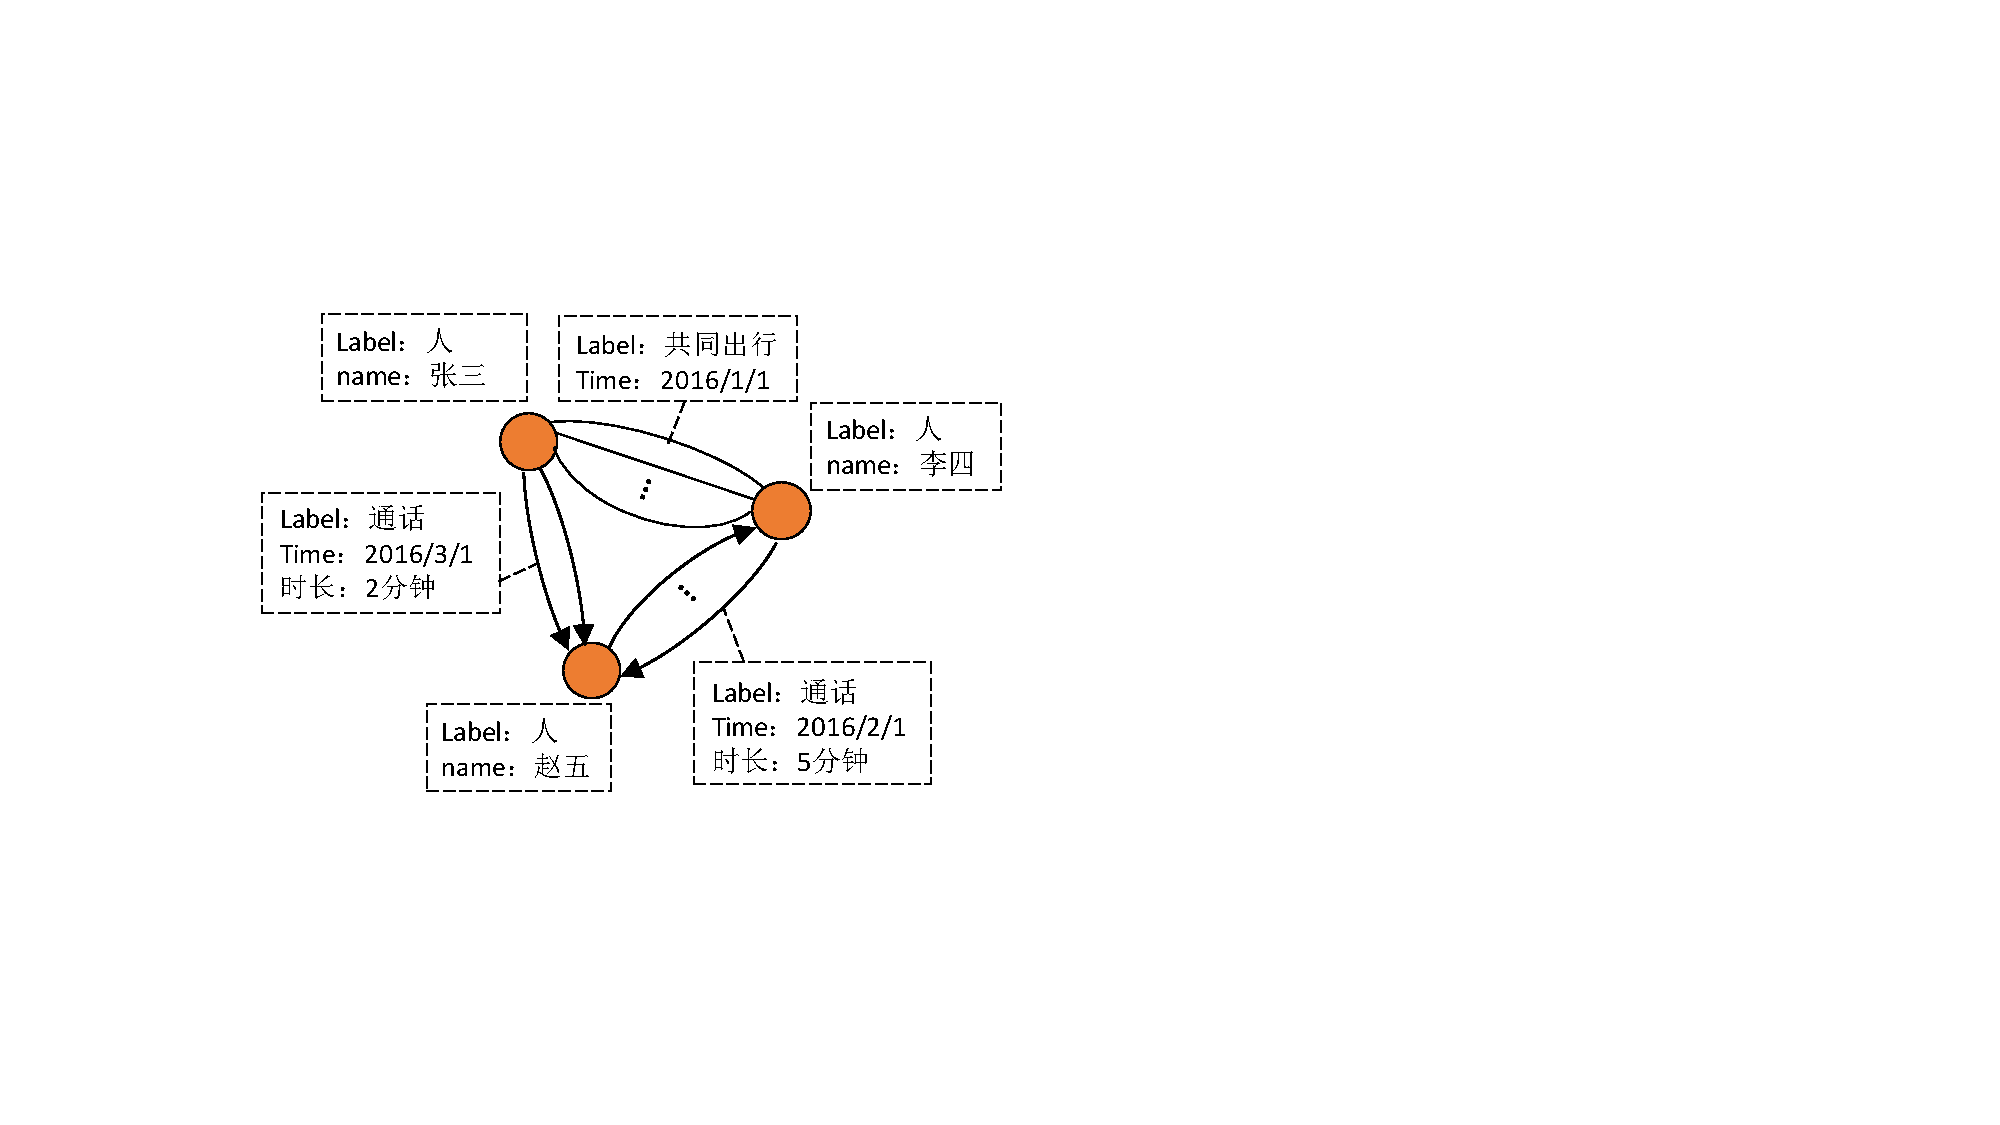
\includegraphics[width=100mm]{fig/property_graph.pdf}
\caption{属性图示例}
\label{fig:property_graph}
\end{figure}

传统解决方案将数据存储在关系型数据库中,如将所有通话数据存储在通话关系表中。关系型数据库能胜任图数据的存储,也能方便地检索元素的内容,但在图结构相关的查询上表现欠佳。比如两跳邻域查询,锁定一个嫌疑人后,要查看其两跳范围内的子图信息。为得到第二跳的邻域结点,需要对各种关系表做昂贵的JOIN操作。图数据库由于其以图的形式存储数据,在图的拓扑结构查询中具有更优异的性能。因此当应用场景中图的拓扑结构查询与元素的内容查询同等重要时,图数据库是最佳的选择。明略数据 是一家大数据解决方案提供商,客户群涵盖刑侦、金融、电信等领域。其中SCOPA 是明略数据的重要产品,在海量刑侦数据上构建起一个数据分析挖掘平台,展现给领域专家的是一张属性图,关联了客户原有的所有数据。SCOPA平台即使用图数据库实现其存储核心。
然而,在富含重边的属性图中,图数据库的查询性能不佳。在传统的图应用中,图中的边一般是稀疏的。如一些公开的图数据集 中,边集的大小约为点集大小的十几倍。但在富含重边的应用场景中,边集大小可能为点集的上万倍。图数据库以邻接表的方式存储图,表中的每一项存储一条边。这使得查询邻接点集时,需要遍历整个邻接表中的所有边。当图中含有大量重边时,邻接表规模巨大,这种数据组织方式导致邻域查询性能严重受损。而邻域查询是大部分图查询的基础,如多跳邻域查询、路径查询、局部聚集系数查询(计算)等,这些查询往往由嵌套的邻域查询实现,随着邻域深度的增加,这种性能受损将被指数级放大。
一种简化重边的建模方式是,将所有同label的重边合并为一条边来表示,边上存储这些重边的所有信息,这样两个实体间的重边数能降低为边的label种类数。然而,将多条重边的数据合并在一条边中存储,会使边的单位数据量骤增,图中的数据粒度过大,同时降低了单条重边的检索和插入效率,每次操作都要先读取相关的所有重边数据,再在其中做查询或插入操作。因此,处理大量重边是一个不可避免的需求。
在许多富含重边的图应用场景中,尽管数据量较大,但数据的操作需求相对单一,而且没有很强的事务性要求。比如在知识图谱的构建中\supercite{knowledge_graph},信息的来源是可靠的,即一旦信息进入知识图谱,则被认为是无需修改的,因此数据操作只需要插入和查询,更新操作很少被执行。在SCOPA的刑侦应用场景中,数据来源是可靠的,且图中数据都是一些客观的事实数据,不需要修改,数据操作主要是图查询和批量的图数据插入。数据插入操作包括原始的全量数据导入和定期的增量数据导入,没有并发的写冲突,也不需要很强的事务性要求。基于上述观察,在放宽了对强事务的支持后,我们可以设计一个相比传统图数据库更为高效的属性图处理系统,来应对含有大量重边的应用场景。
本文提出了一种基于图数据库Titan 和列式存储数据库HBase 的复合存储架构——HybriG。HybriG能从容地处理富含重边的属性图,克服图数据库的局限性,具有更好的查询和插入性能。HyBriG架构应用于SCOPA的底层核心设计,在实践中也验证了其性能的优异性。本文的贡献主要有:分析了图数据库处理大量重边时性能受损的原因,并基于此提出了解决方案HybriG及其存储、查询和高效数据导入设计,最后通过实验验证了HybriG的优异性能。
本文组织如下:第2节介绍图数据库相关的预备知识,包括HBase及Titan的实现及其在处理大量重边时的局限性;第3~6节介绍HybriG的系统架构,包括查询模块的设计,数据高效导入方案的设计,以及数据一致性的设计;第7节展示实验结果。第8节介绍大规模图数据处理的相关工作。最后在第9节对本文进行总结。


% vim:ts=4:sw=4

	% 各章节。
	% Copyright (c) 2014,2016 Casper Ti. Vector
% Public domain.

\chapter{相关工作}  \label{chap:related}
\section{分布式数据库HBase}
HBase是Google BigTable\supercite{bigtable}的开源实现 ,是Hadoop 生态系统中一个列式NoSQL数据库,搭建在HDFS(Hadoop分布式文件系统)之上。HBase由于其优异的可扩展性和稳定性,在产业界得到了广泛应用。HBase也是图数据库Titan最常使用的存储引擎,为了介绍Titan的底层实现,此处先详述HBase的相关实现。
下面分别介绍HBase的数据模型、操作接口、存储实现以及HBase与同类系统的对比。

\subsection{HBase数据模型}
在HBase中,数据首先以表为单位进行组织。数据表以行为单位组织,每行由一个键值唯一标识,称为行键(row key)。一行中可以包含任意列的数据,每列对应的数据可分为多个版本(对应多个时间戳)。每个版本的数据是最小粒度的数据单元,称为一个单元格(cell)。因此一个单元格由行键、列名、版本号(时间戳)和值(value)组成。
在HBase中,各列按列族(column family)进行组织,因此列名实际由列族名和列修饰符(column qualifier)组成。区别于传统关系模型,列族里的列修饰符可以随时添加,不需要事先定义。即在插入数据时,可以指定任意的列修饰符。行键是每个表必须要有的一列,且只能是唯一的一列,不属于任何列族。图\ref{fig:hbase_table}是HBase中一张数据表的示例。

\begin{figure}[htbp]
\centering
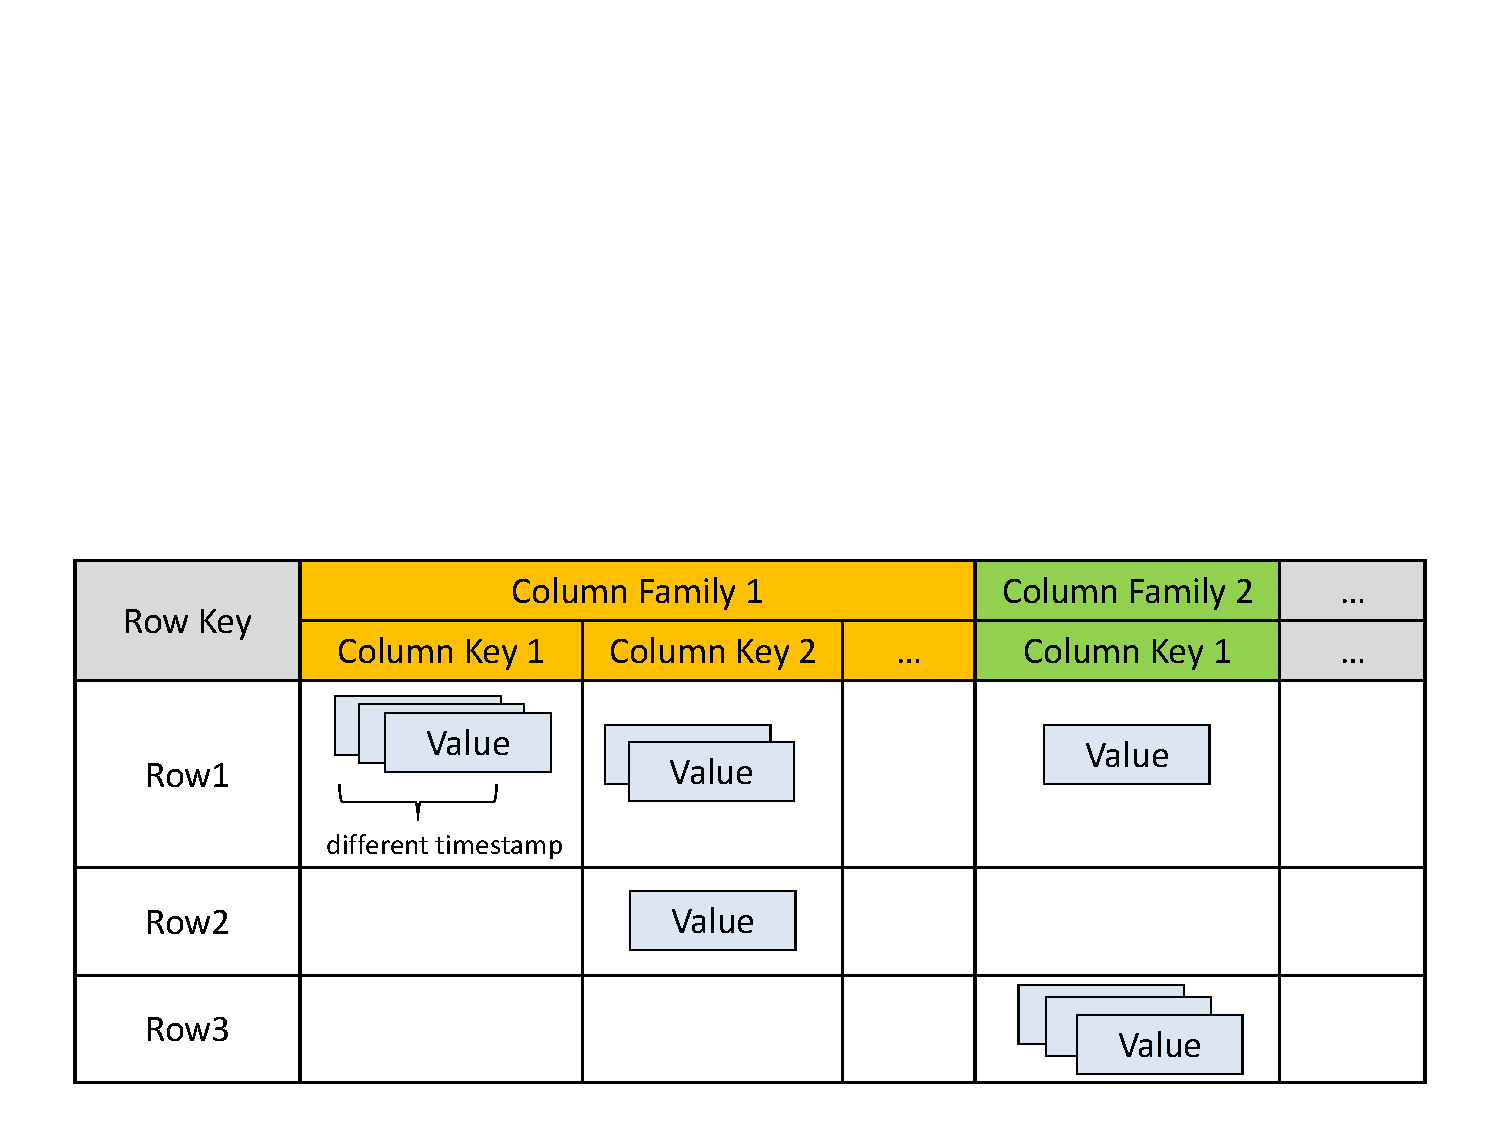
\includegraphics[width=120mm]{fig/HBase_table_example.pdf}
\caption{HBase数据表示例}
\label{fig:hbase_table}
\end{figure}

HBase也被认为是一个键值存储(Key-Value Store),相当于数据结构Map的存储。这是因为每个单元格实际存储的是Value部分,而Key部分就是由行键、列族名、列修饰符和时间戳合并构成。由于列修饰符是不需要事先定义的,因此整个Key部分是可以随意指定的,从而可以将HBase归类为键值存储。图\ref{fig:hbase_cell}是一个Cell的数据组成以及如何表示为键值对的示例。单元格也确实是HBase的存储实现中的最小单元,因此将HBase归类为键值存储。

\begin{figure}[htbp]
\centering
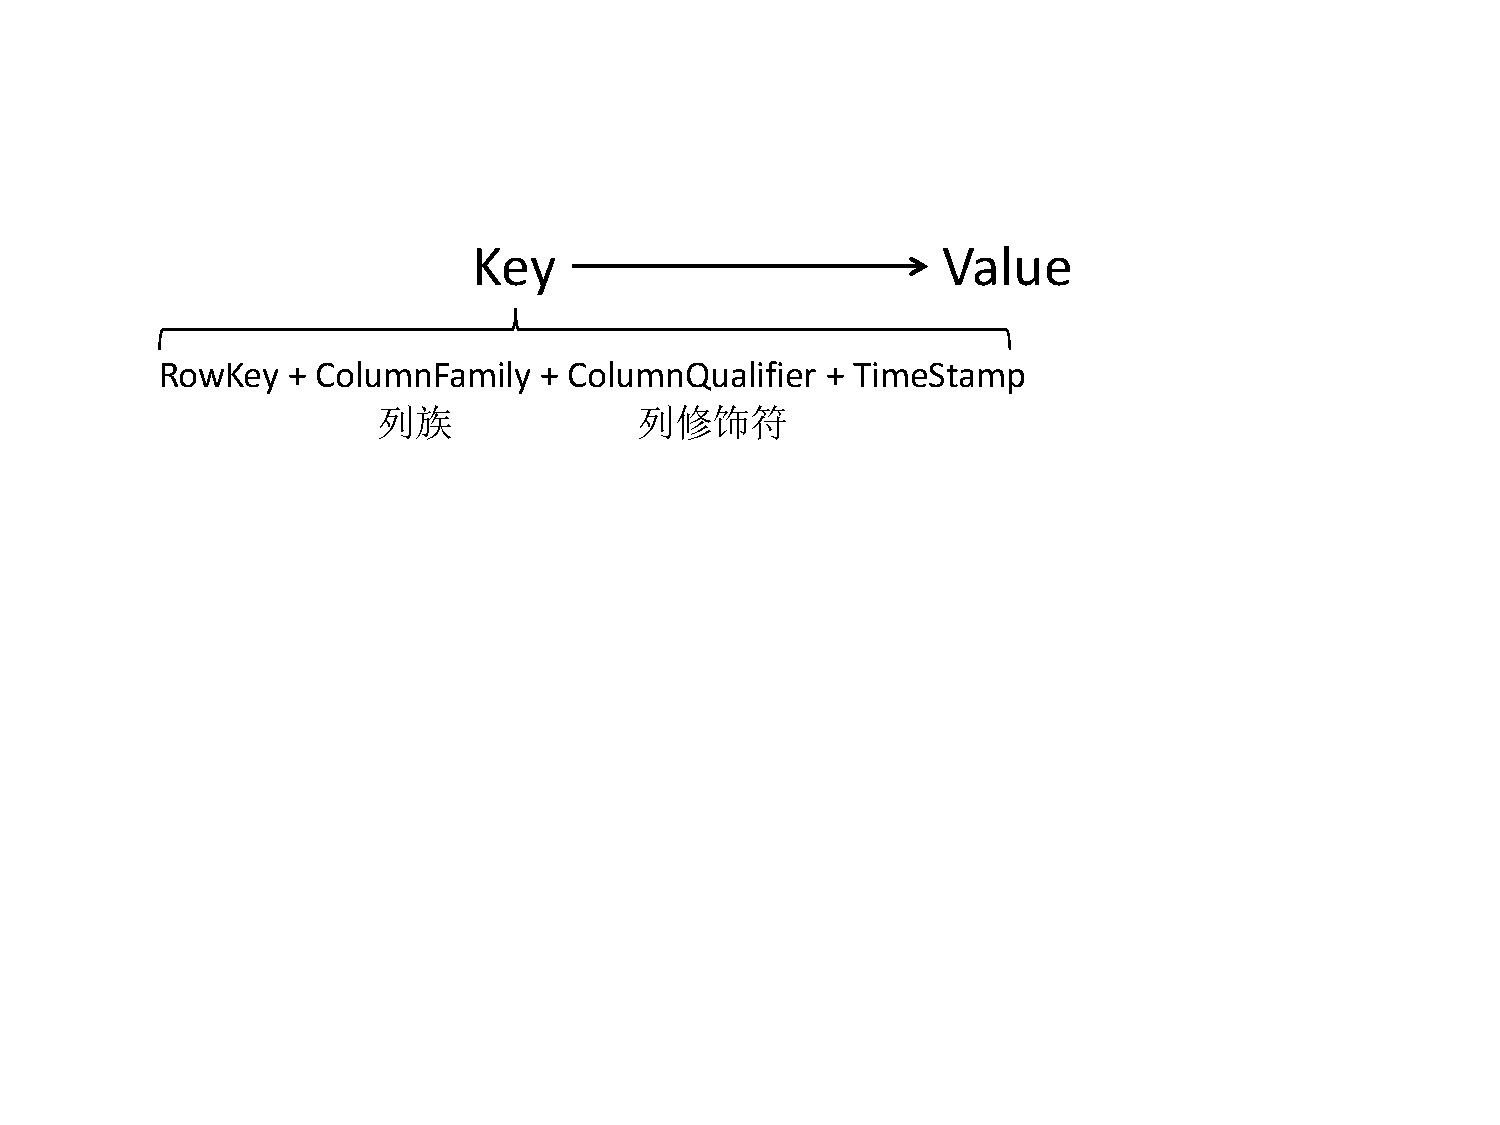
\includegraphics[width=120mm]{fig/HBase_key_value.pdf}
\caption{HBase中Cell单元的Key、Value成分}
\label{fig:hbase_cell}
\end{figure}

\subsection{HBase操作接口}
HBase提供了一个交互式的shell作为操作接口,同时也提供原生的Java接口,另外还提供了thrift API,支持C++、Python、Ruby、Perl、PHP等语言。下面以HBase shell为例叙述HBase的操作接口。

HBase建表时需要指定表中的所有列族,下面的操作创建了名为table1的数据表,它拥有两个列族cf1和cf2:
\begin{lstlisting}
HBase Shell > create 'table1', 'cf1', 'cf2'
\end{lstlisting}

在建表之后还可以增加或删除列族,也可以修改列族的配置,但需要disable整个表,即中止所有读写请求,操作结束后再enable该表:
\begin{lstlisting}
HBase Shell > disable 'table1'
HBase Shell > alter 'table1', {NAME => 'cf2', VERSIONS => 5}
HBase Shell > alter 'table1', 'delete' => 'cf1'
HBase Shell > alter 'table1', 'cf3'
HBase Shell > enable 'table1'
\end{lstlisting}
上面的操作设置列族cf2的最大版本数为5,即每列最多存储5个版本的数据。下一行删除列族cf1及其下的所有数据。之后添加一个列族cf3。

HBase提供Put、Get、Scan、Delete接口进行数据的增删查改。Put接口给某一行中插入一个单元格,需要指定行键、列族和列修饰符。时间戳则是可选的,若没有指定,则使用插入时间作为时间戳。
\begin{lstlisting}
HBase Shell > create 'table1', 'cf1', 'cf2'
HBase Shell > put 'table1', 'row1', 'cf1:a', 'value1'
HBase Shell > put 'table1', 'row2', 'cf2:b', 'value2'
HBase Shell > put 'table1', 'row1', 'cf1:b', 'value3', timestamp1
\end{lstlisting}

Delete接口跟Put接口相反,用来删除一个单元格的数据。由于参数相同,这里不再举例。

Get接口跟Scan接口用来读取数据,其中Get接口用来读取一行内的数据,Scan接口用来读取多行的数据。Get接口只需给定一个行键,参数里的列族、列修饰符和时间戳都是可选的,会把满足条件的所有单元格都返回。Get接口能读取的范围不超过一行,即Get接口可以读取一个单元格,也可以读取一行中所有的单元格,但读取的对象都只能在同一行中。下面是一些读取示例:
\begin{lstlisting}
HBase Shell > get 'table1', 'row1'
HBase Shell > get 'table1', 'row1', 'cf2:a'
HBase Shell > get 'table1', 'row1', {COLUMN => ['cf:a', 'cf:b', 'cf:c']}
HBase Shell > get 'table1', 'row1', {COLUMN => 'cf:c', TIMESTAMP => ts1}
\end{lstlisting}

Scan接口则用来读取连续的多行数据。在HBase数据表中各行是按行键升序排列的,因此Scan时只需给定一个起始行键和一个终止行键(不包含),就可以返回所有的这些行。如果不给定范围,则Scan接口返回表中的所有数据。Scan接口也可指定特定的列或附加Filter来过滤无关数据。下面是一些操作示例:
\begin{lstlisting}
HBase Shell > scan 'table1', {LIMIT => 100}
HBase Shell > scan 'table1', {COLUMNS => ['cf1:a', 'cf1:b'], LIMIT => 10,
                              STARTROW => 'xyz'}
\end{lstlisting}
第一行读取表中的100行数据,第二行从行键大于等于'xyz'的行中读取列族为cf1,列修饰符为a或b的10行数据。

之所以要区分Get和Scan接口,是因为HBase只保证单行数据的原子性,即Get接口不会返回部分更新的数据,但Scan接口没有这个保证。
在本节也可以看到,HBase并没有提供类型关系数据库的SQL接口,这是所有NoSQL数据库的一个特点,都是根据自己的数据模型因地制宜地提供对应的接口。

% ACID的支持情况是否要说?

\subsection{HBase存储实现}
HBase集群采用Master-Slave架构,其中Master节点为HMaster,Slave节点为RegionServer,每台工作机器只需部署一个RegionServer。
HMaster和RegionServer之间通过ZooKeeper\footnote{ZooKeeper, http://zookeeper.apache.org/}来协同工作。HMaster没有单点问题,HBase中可以启动多个HMaster,通过Zookeeper的Master Election机制保证总有一个HMaster在运行。

\begin{figure}[htbp]
\centering
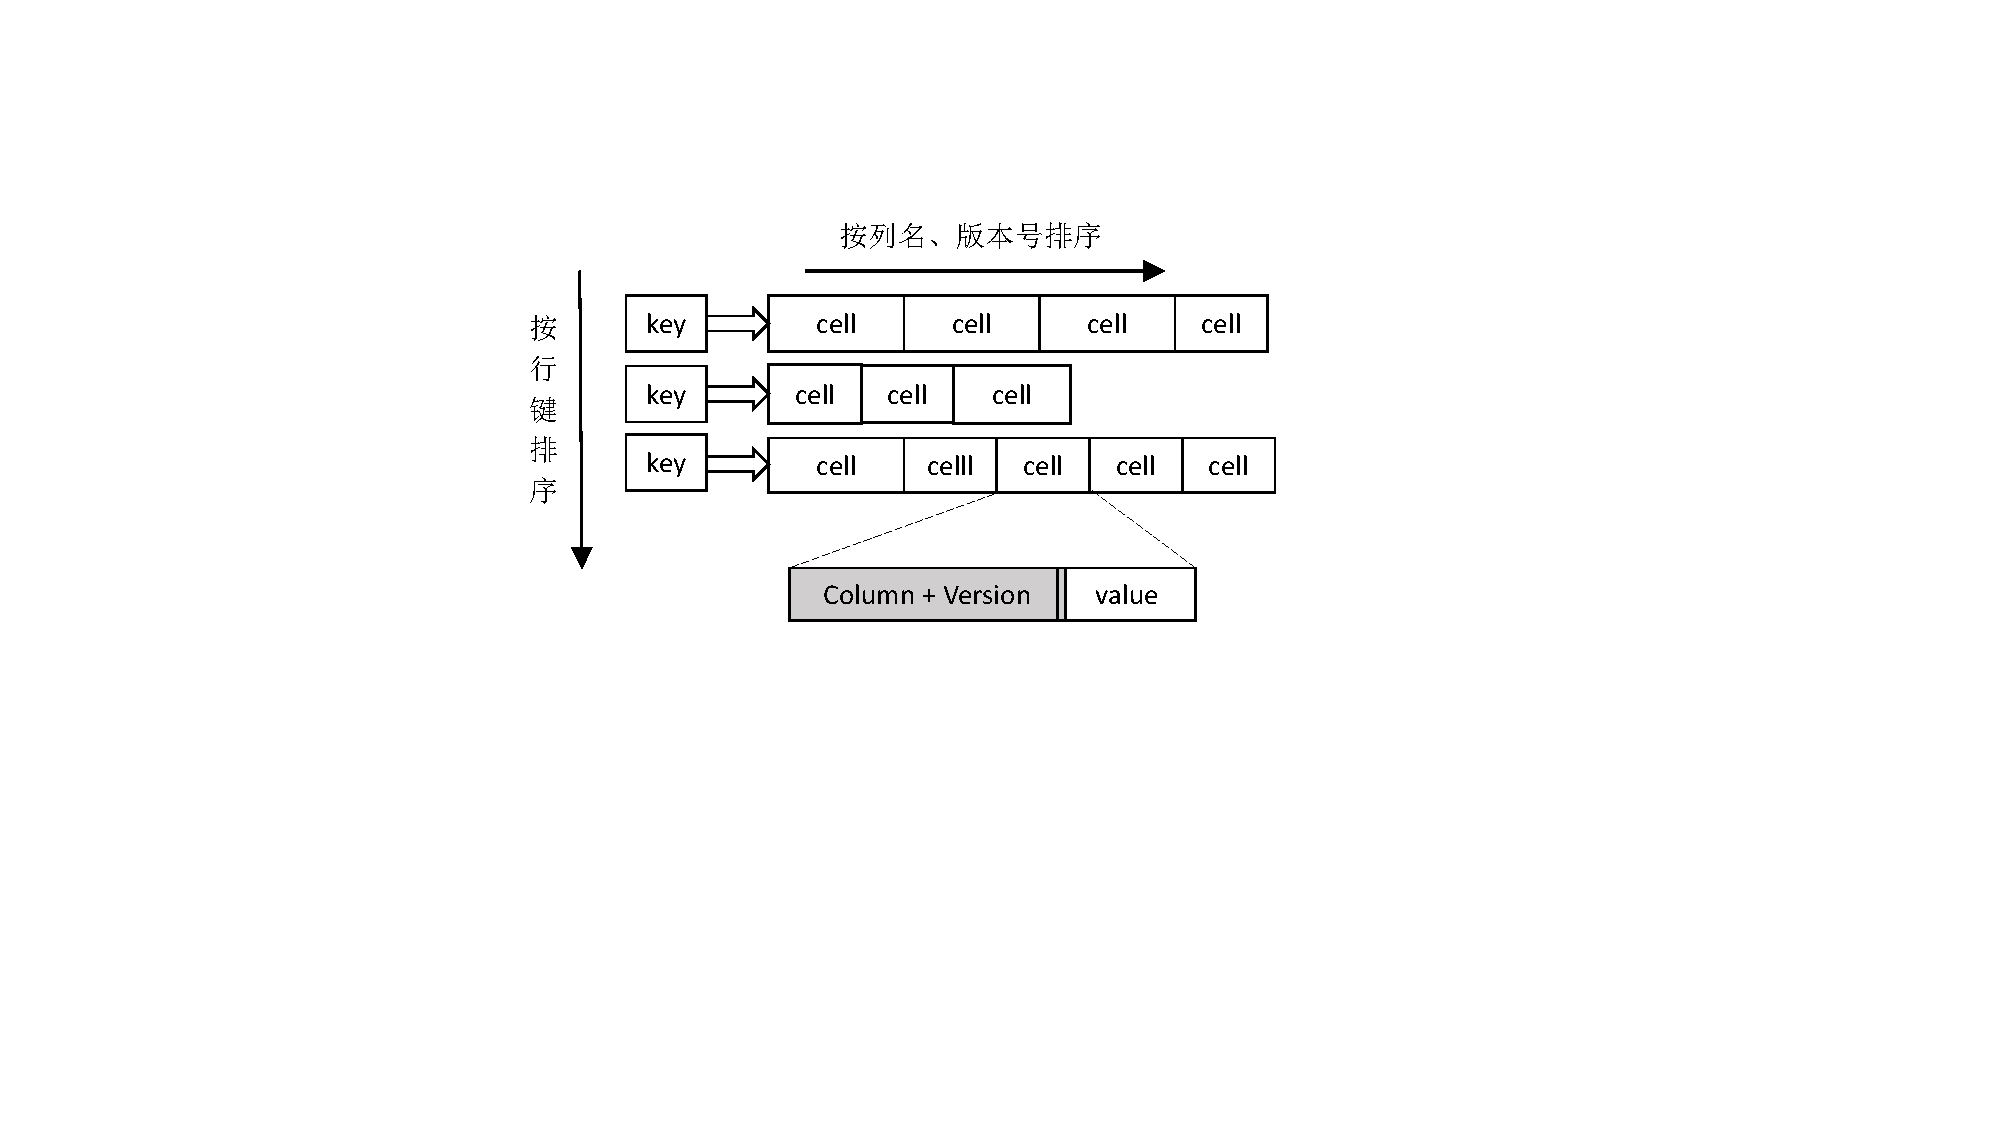
\includegraphics[width=100mm]{fig/big_table.pdf}
\caption{BigTable模型示例}
\label{fig:big_table}
\end{figure}

RegionServer负责管理数据表的分片(Region)。HBase采用BigTable数据模型(如图\ref{fig:big_table})。在BigTable数据表中,各行首先按行键升序排列,行内的各单元格再依次按列名、时间戳排序。作为一个列式存储数据库,HBase中不同列族的数据是分开存储的。由于行键有序,因此可以装数据表水平切分为不相交的Region,每个Region由一个左闭右开的行键区间来表示。每个Region交由一个RegionServer来管理,RegionServer进一步将这些数据存储在HDFS中,并响应这个Region上的读写请求。

\begin{figure}[htbp]
\centering
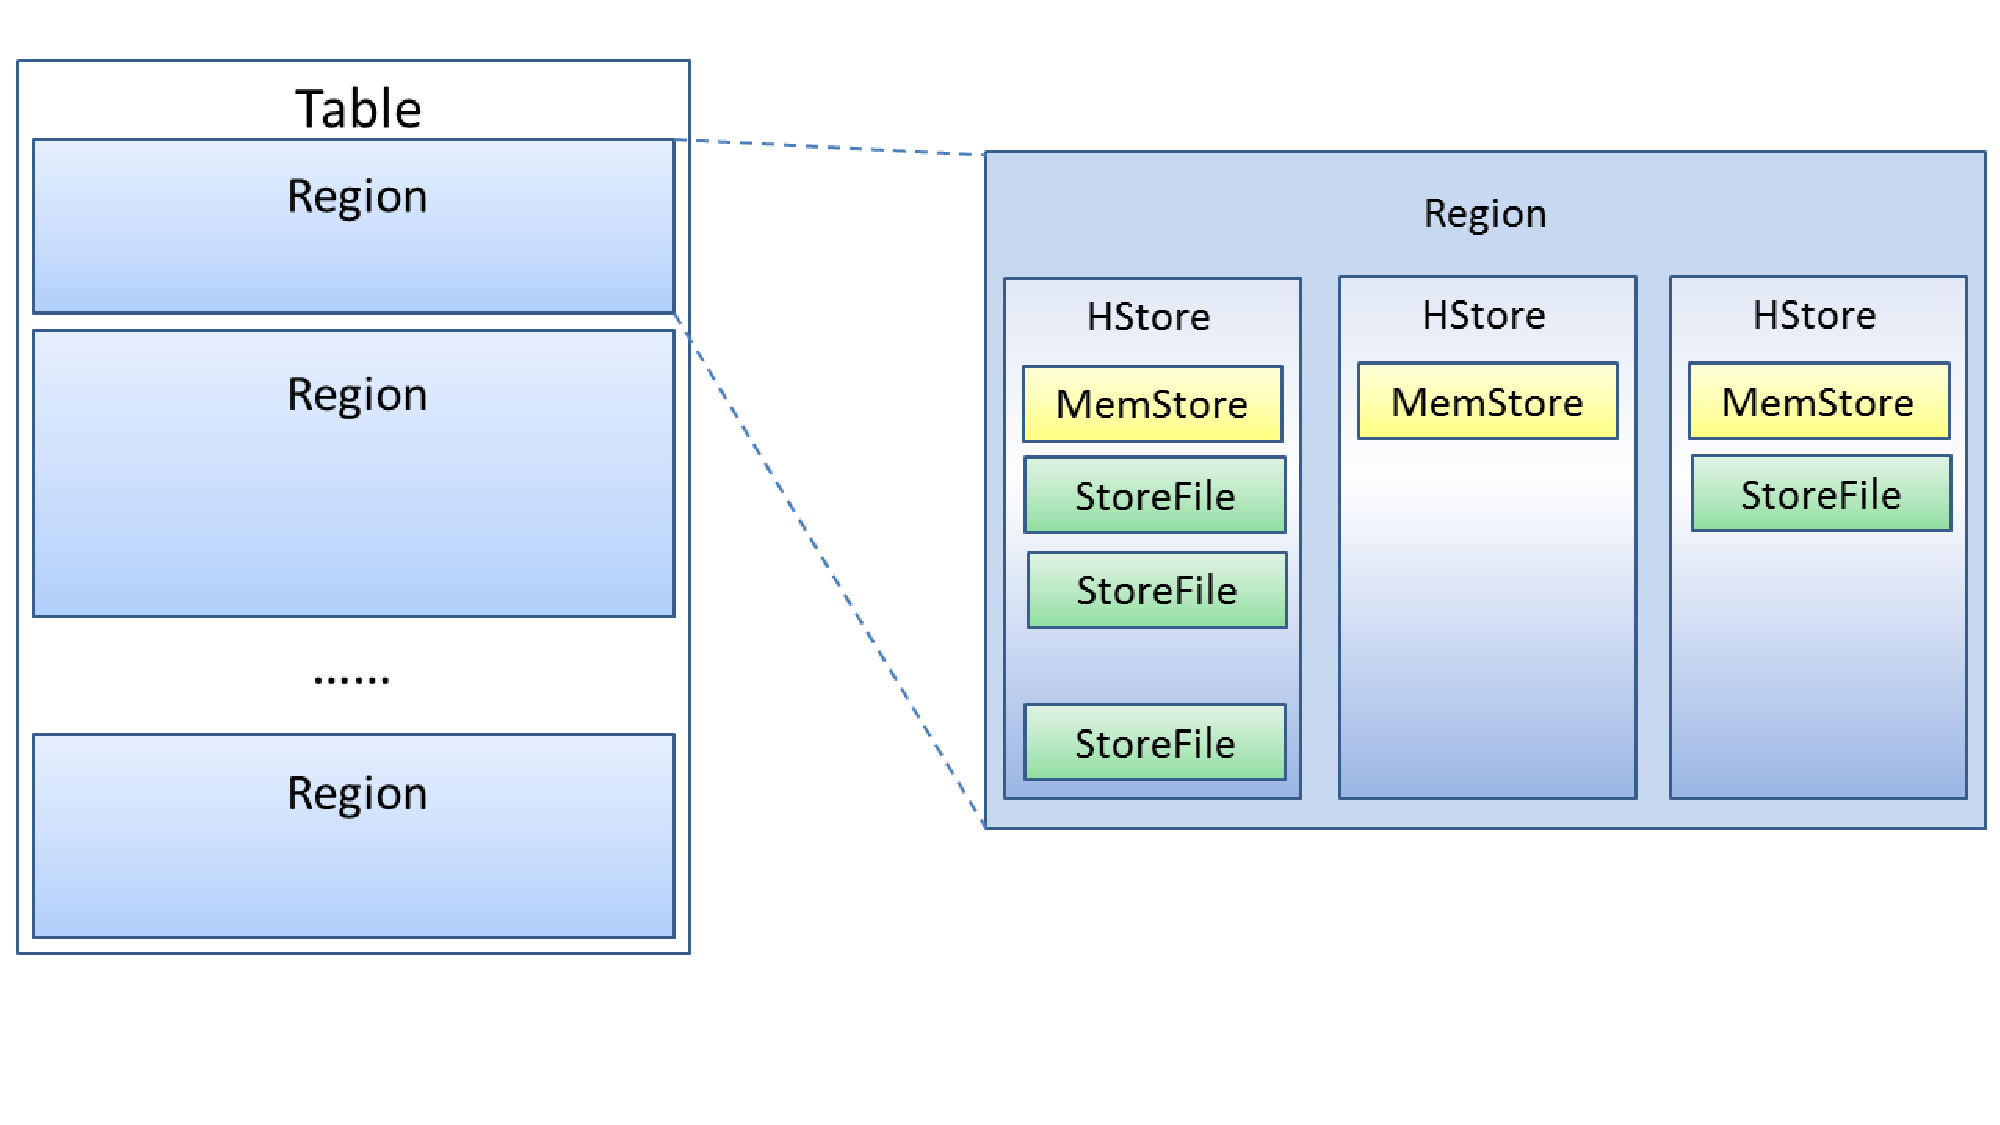
\includegraphics[width=120mm]{fig/HBase_region.pdf}
\caption{HBase Region内部结构}
\label{fig:hbase_region}
\end{figure}

每个Region在RegionServer内的组成成分如图\ref{fig:hbase_region}所示。
Region内部先按列族分为不同的HStore,每个HStore采用LSM Tree\supercite{LSM_tree}数据结构进行存储。在LSM Tree中,数据更新先写入内存缓冲区MemStore中,在MemStore中数据是有序排列的。当MemStore写满时,会将数据flush进磁盘成为文件,即一个StoreFile。由于生成StoreFile时是磁盘的顺序写,因此具有很高的性能。HBase利用LSM Tree数据结构实现了高效的随机写入。然而给定一个Key值要进行读取时,需要在MemStore和所有StoreFile中进行查找,如果StoreFile数目过多将会影响读取速度。RegionServer有线程会定期对HStore里的StoreFile进行合并(compaction),以降低StoreFile的数目,减小读请求的开销。

最后需要补充的是,每个RegionServer会维护一个WAL(Write Ahead Log)文件,写请求在写入MemStore前都需要先写入WAL中,以保证宕机时内存中的数据不会丢失。WAL和底层的StoreFile都是存储在HDFS上的,具有多复本的容错机制。当某台 RegionServer 宕机时,HMaster会将这些文件分配给其它RegionServer进行恢复,从而实现容错性(Fault Tolerance)。

\subsection{HBase与同类系统对比}
在分布式键值存储中,另一个著名的系统是Cassandra\supercite{cassandra}。Cassandra是Amazon DynamoDB\supercite{DynamoDB}的开源实现,最初由Facebook开发并开源。

在存储实现方面,区别于BigTable中按字典序来划分Key值空间的实现,Cassandra中是按Key值的哈希值来划分空间的。另外Cassandra不依赖于HDFS进行存储,其数据直接由各Server存储在本地磁盘中,Server之间对数据保留多个复本。由于Key值的寻址逻辑更为简单,以及更为直接的存储实现,Cassandra相比HBase具有更优的读写性能。

在系统架构方面,Cassandra使用去中心化的系统架构,没有Master节点,因此完全除去了单点故障的可能。所有Server组成一个环状结构,使用一致性哈希算法来分配Key值空间。一致性哈希算法使得集群可以方便地添加或删除节点。区别于HBase依赖ZooKeeper进行协作,Cassandra中的Server之间使用Gossip协议进行协作。

Cassandra与HBase最大的区别在于CAP\supercite{CAP}理论上的取舍。CAP是Consistency、 Availability、 Partition tolerance的简称,表示分布式系统的三个性能。Consistency是指系统的读请求总能返回最新的写结果,即读写请求是一致的。Availability是指系统一直处于可用的状态,不会因为宕机等原因造成一段时间不可服务。Partition tolerance是指分布式系统因网络故障等被切分为不可通信的几部分时仍能正常工作。CAP理论指出,任何系统最多只能满足三条性能中的两条,不可能三者兼备。

HBase和Cassandra都是分布式的系统,在部分机器宕机或失联时系统仍能工作,都是满足Partition tolerance的。它们的区别在于Consistency和Availability的取舍上。
HBase 在有RegionServer宕机时,需要让相应的WAL和StoreFile在其它RegionServer上进行恢复,在恢复期间对应的Region是无法提供服务的,因此不满足Availability。但也正得益于这种恢复机制,HBase中的数据会一直处于一致的状态,即HBase满足Consistency。
Cassandra由于不依赖HDFS之类的可靠存储层,需要自身在各Server间对数据做多复本存储。而读请求是可以由单独一台Server来响应地,不需要等待各Server间的同步,因此也就没有了一致性的保证,按来了读写的高性能。

\section{图数据库Titan}
图数据库是以图的形式来表示和管理数据的数据库\supercite{graph_models_survey},与传统的关系型数据库相比,图数据库在图结构相关的查询上有更优异的性能,如多跳邻域查询、路径查询、局部聚集系数计算等。
Titan是一个基于Blueprints\footnote{Blueprints, https://github.com/tinkerpop/blueprints/wiki} 接口设计的开源图数据库。Blueprints是属性图数据库的一套标准,类似于关系数据库里的JDBC,大部分图数据库都实现了Blueprints接口。

\begin{figure}[htbp]
\centering
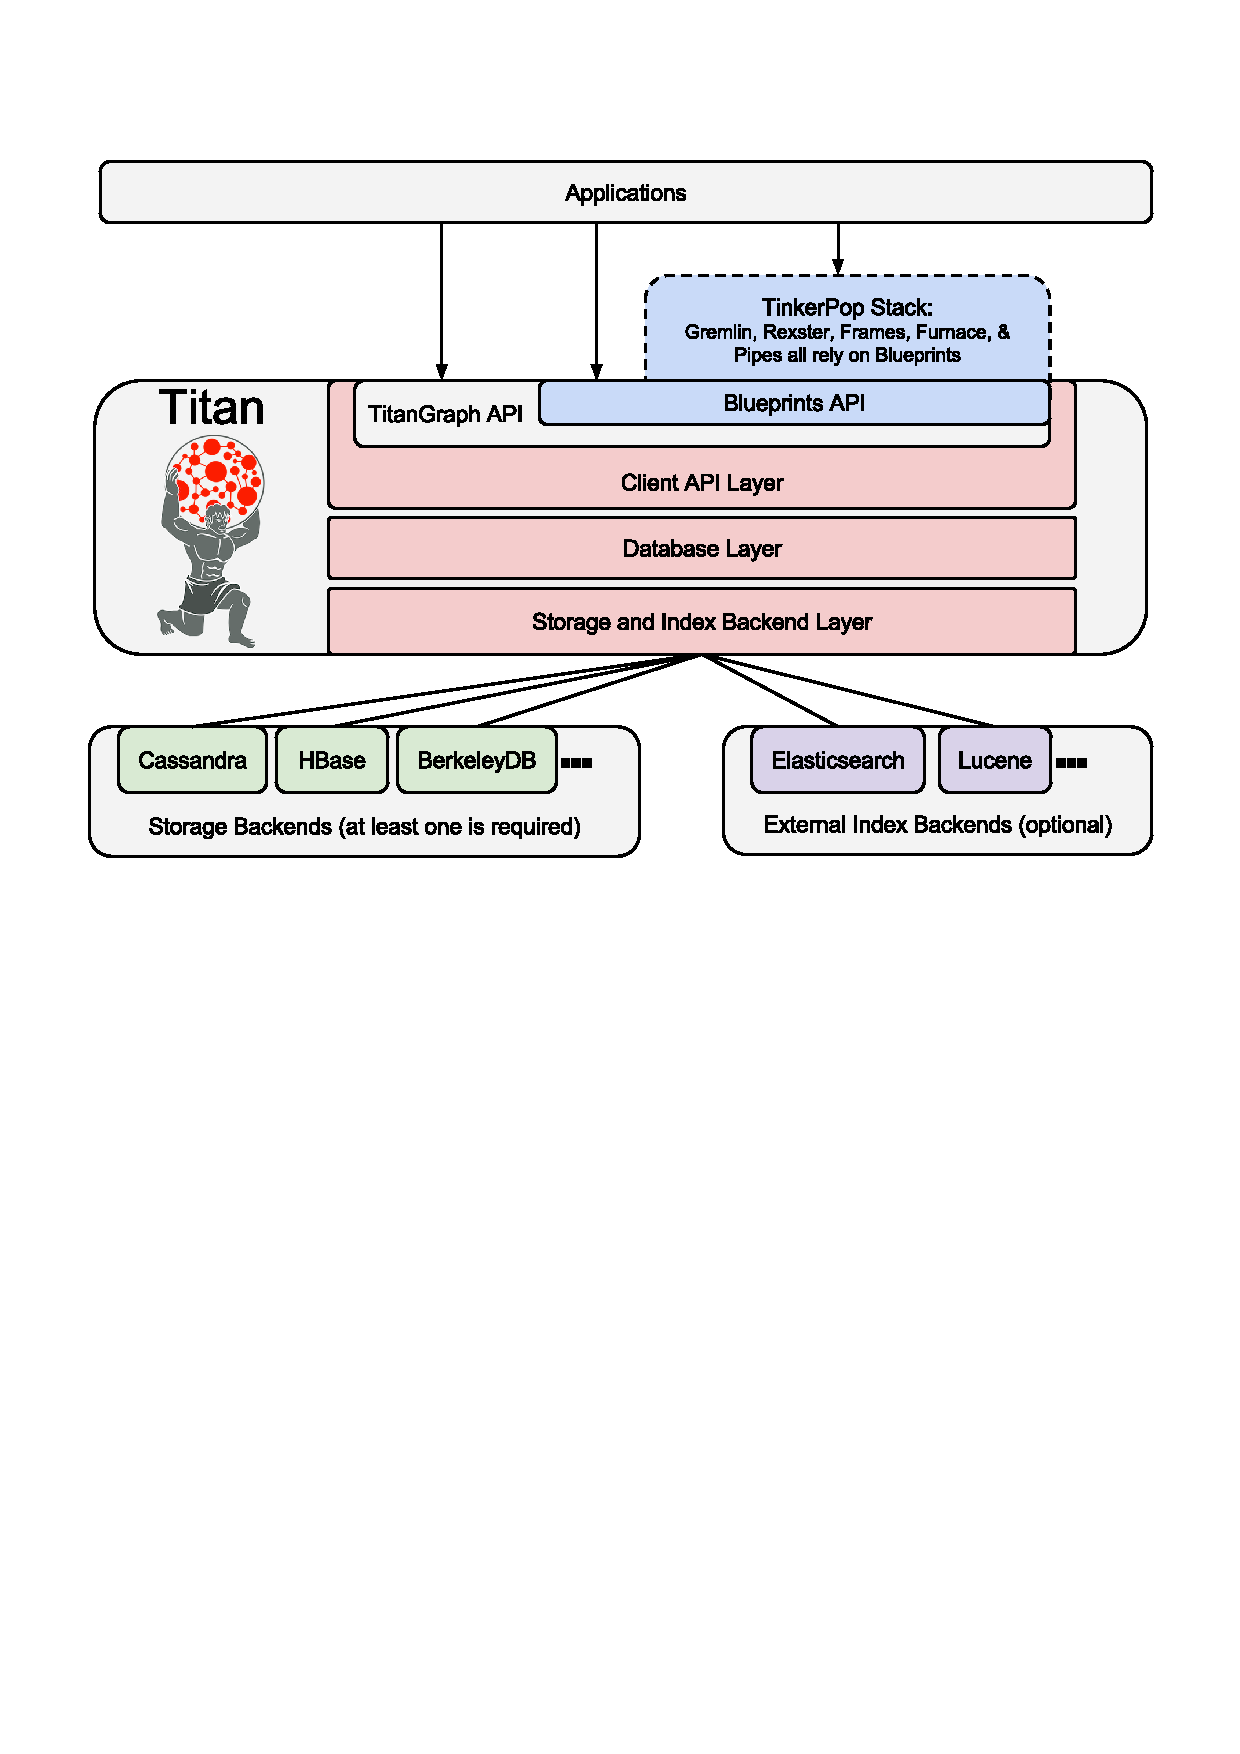
\includegraphics[width=140mm]{fig/titan-architecture.pdf}
\caption{Titan架构图}
\label{fig:titan_arch}
\end{figure}

Titan实现了可插拔的存储接口,可以部署在BerkerlyDB 、HBase或Cassandra之上 ,即Titan不会自己管理数据,其数据存储在底层的存储引擎之中。Titan在索引方面也提供了可插拔的接口,因为Titan只利用存储引擎实现了精确匹配的索引(类似倒排索引),更高级的索引需要依赖索引引擎来实现。Titan支持的索引引擎有ElasticSearch、Lucene等。图\ref{fig:titan_arch}是Titan架构图\footnote{图片来源:http://s3.thinkaurelius.com/docs/titan/0.5.4/images/titan-architecture-layer-diagram.svg}。

相比于著名的图数据库Neo4j,Titan是完全开源免费的,其受关注度正在与日俱增。而且由于Hadoop生态系统在产业界的广泛应用,在HBase上搭建Titan,即使用Titan on HBase应对图处理需求是较为常见的选择。下面分别介绍Titan的操作接口、Titan的存储实现,以及Titan在处理大量重边时的局限性。

\subsection{Titan操作接口}
\subsubsection{Schema设置(DDL接口)}
图的Schema包括edge labels、vertex labels和property keys等。Property key是指某种属性的Key值,如"name"、"gender"、"age"等。label是点和边的标签,可以认为是一种特殊的属性,但每个元素只能有一个label。这些都需要在使用前事先定义。

定义点的label只需要给定一个label名,后续在添加点时,需要指定使用的是哪个vertex label。下面是操作示例:
\begin{lstlisting}
mgmt = g.getManagementSystem()
person = mgmt.makeVertexLabel('person').make();
mgmt.commit()
// Create a labeled vertex
person = g.addVertexWithLabel('person')
// Create an unlabeled vertex
v = g.addVertex(null)
g.commit()
\end{lstlisting}

Edge label的定义需要给出lable名,以及边的重复度限制(Multiplicity)。
Multiplicity 有 MULTI、 SIMPLE、 MANY2ONE、 ONE2MANY、 ONE2ONE 五种取值。其中 MULTI 表示这种类型的边可以在两点间连任意多条,即本文研究的重边。 SIMPLE表示两点间最多只能连一条这样的边,比如好友关系,如果两人之间有好友关系,则连一条这样的边,否则不连。加上 SIMPLE 类型使得两人之间不能连多条表示好友关系的边。MANY2ONE 表示每个点至多只有一条这样的出边,但是对该label的入边数目没有限制。比如表示mother关系(母子关系)的边,一个人只能有一个母亲,但一个母亲可以有多个孩子。 ONE2MANY 的意义与 MANY2ONE 相反,每个点至多只有一条这样的入边。 ONE2ONE 表示这种边是一对一的,即两个点之间如果连了一条这样的边,这两个点就不能再跟任何其它点有这样的边相连。比如夫妻关系,就是 ONE2ONE的 例子。下面是创建edge label的示例:
\begin{lstlisting}
mgmt = g.getManagementSystem()
follow = mgmt.makeEdgeLabel('follow').multiplicity(Multiplicity.MULTI).make()
mother = mgmt.makeEdgeLabel('mother').multiplicity(Multiplicity.MANY2ONE).make()
mgmt.commit()
\end{lstlisting}

Property key的定义需要给出key的名称,以及数据类型,还有数据的基数(Cardinality)。 Cardinality有 SINGLE、 LIST、 SET 三种选择。 SINGLE就是最普通的 key-value对,即value部分只会填一个单一的值。 LIST是指value部分是一个列表,对value部分的操作将是添加或删除部分值。 SET则表示value部分是一个去重的值的集合。下面是一些操作示例:
\begin{lstlisting}
mgmt = g.getManagementSystem()
birthDate = mgmt.makePropertyKey('birthDate').dataType(Long.class).cardinality(Cardinality.SINGLE).make()
name = mgmt.makePropertyKey('name').dataType(String.class).cardinality(Cardinality.SET).make()
sensorReading = mgmt.makePropertyKey('sensorReading').dataType(Double.class).cardinality(Cardinality.LIST).make()
mgmt.commit()
\end{lstlisting}

\subsubsection{查询接口}
Titan提供Gremlin\footnote{Gremlin, https://github.com/tinkerpop/gremlin/wiki}查询接口让用户可以在图上进行游走(traversal)查询。Gremlin是基于Blueprints接口实现的一门函数式图查询语言,可以把图查询表示成链式的函数调用,使得代码非常直观。

下面是一个查询示例,查询 name 属性为 hercules的点在 father关系上两跳出边的点的 name属性值。
\begin{lstlisting}
gremlin> g.V.has('name','hercules').out('father').out('father').name
==>saturn
\end{lstlisting}

下面是一个更丰富的查询示例,在找到name为hercules的点后,查询其father、mother出边连接的点的label,查询结果为'god'和'human'。再查询hercules节点所有battled出边所连接的点的label,查询结果是3个邻接节点的label都为monster。最后一个查询显示所有battled出边所连接的点的所有属性。每个点只有一个key值为name的属性,因此每行中只有一个key value对。
\begin{lstlisting}
gremlin> hercules = g.V.has('name','hercules').next()
==>v[1536]
gremlin> hercules.out('father','mother')*.getVertexLabel()
==>god
==>human
gremlin> hercules.out('battled')*.getVertexLabel()
==>monster
==>monster
==>monster
gremlin> hercules.out('battled').map
==>{name=nemean}
==>{name=hydra}
==>{name=cerberus}
\end{lstlisting}

Gremlin也可以表达一些复杂的查询条件,如给定两个点v1和v2,查询它们之间的所有边:
\begin{lstlisting}
gremlin> v1.bothE   // get all edges of v1
gremlin> v1.bothE.filter{it.outV.next() == v2 || it.inV.next() == v2}
\end{lstlisting}
第一行的查询将返回v1的所有出边和入边。第二行的查询则在所有边的基础上加了个filter,接收一个表达式(Closure)作用在迭代器上,迭代器it每次指向一条边,判断它的端点是否包含v2,如果包含则表明是v1和v2共用的边。因此第二行返回v1、v2相连的所有边。


\subsubsection{数据操作接口(DML接口)}
用Gremlin在图中插入点和边是很方便的,下面是一个插入数据的示例:
\begin{lstlisting}
alice = g.addVertexWithLabel("person")
alice.setProperty("name", "Alice")
bob = g.addVertexWithLabel("person")
bob.setProperty("name", "Bob")

e = alice.addEdge("isFriend", bob)
e.setProperty("since", 1991)
g.commit()
\end{lstlisting}
g是一个TitanGraph对象,第1、2行往图中插入一个label为"person"的点,并设置属性"name" 为"Alice" ,第3、4行类似地插入一个表示Bob的点。第6、7行在这两个点间连一条label为 "isFriend"的边,并设置边上的属性。最后第8行需要执行commit,以将修改持久化到存储中。同时这也表示当前事务的结束,在Titan中,对图(即对象g)的初次操作将打开一个Thread Local的事务,只有执行commit才能结束当前事务。

更详细的Gremlin接口介绍,可参见Gremlin文档\footnote{GremlinDocs, http://gremlindocs.spmallette.documentup.com/}。

\subsection{Titan存储实现}
在图数据库Titan中,基于BigTable模型,数据在HBase中以邻接表的形式存储,如图\ref{fig:adj_list}所示。

\begin{figure}[htbp]
\centering
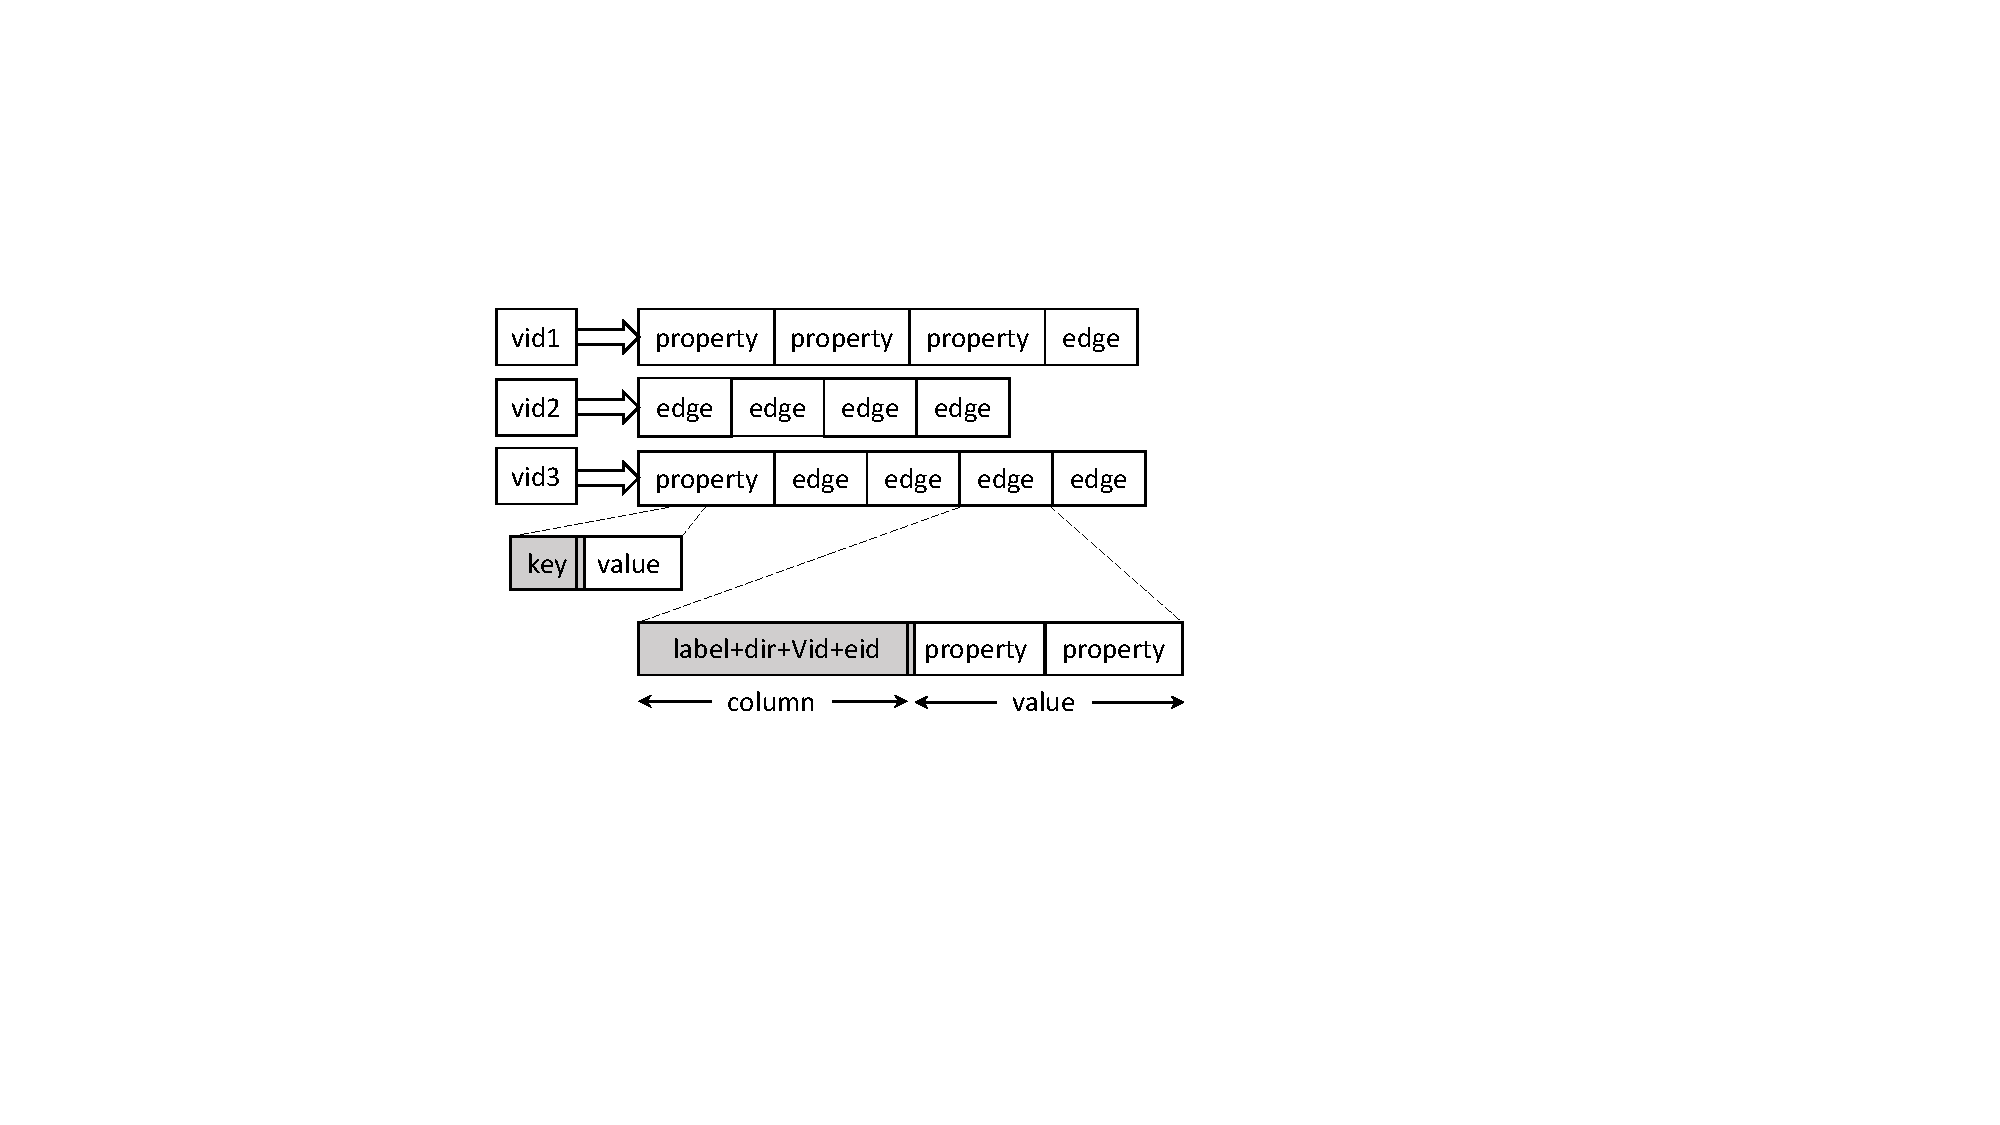
\includegraphics[width=100mm]{fig/adj_list.pdf}
\caption{Titan图数据内部的BigTable表示}
\label{fig:adj_list}
\end{figure}

Titan为每个点分配了一个全局唯一的id,每个点占BigTable中的一行,行键就是点的id。每行存储了该点相关的属性和边,它们各占一个单元格。边和属性数据都存储在一个列族之中,并设置该列族的最大版本数为1,从而使每行中的列修饰符与单元格一一对应,根据行键和列修饰符可以唯一定位到目标单元格,实现对边和属性内容的快速检索。

在Titan中,每个属性是一个key-value对。点的属性存储在该点所在的行,每个属性占一个单元格,并以属性名key作为列修饰符,这使得每个点的属性查询可以非常高效。下面的代码展示了点的属性查询对应的HBase Shell操作,其中"graph\_tbl"是一张图在HBase中的数据表的表名;vid是该点的id,作为行键;边集数据和属性数据所在的列族名为"e"。
\begin{lstlisting}
// Gremlin Command
v.getProperty("name")
// HBase Shell Command
hbase shell> get "graph_tbl", vid, "e:name"
\end{lstlisting}

每个点所在的行还存储了邻接的所有边数据,每条边占一个单元格。一条边的信息包含了邻接点、类别(label)、方向、边的唯一id,以及边上的各属性。单元格的值用来存储边上的所有属性,列修饰符则存储边上除属性外的其它信息。在BigTable模型中,同一行的单元格按列名排序。为了方便检索,每条边所在的单元格依次以label、方向、邻接点id以及边id拼接成为列名,即
\begin{equation}
  \mbox{列修饰符} = \mbox{边}label + \mbox{方向} + adjVid + eid \label{eq:cq_design}
\end{equation}
这种列名设计使得一个点的所有边先按label排序,再按方向、邻接点id、边id等排序。其优点是当要检索该点指定label的所有边时,只需要扫描邻接表的一部分。图\ref{fig:orginal_list}是一个更详细的示例。下面的代码展示了点的边集查询对应的HBase Shell操作。

\begin{lstlisting}
v.getEdges()
hbase shell> get "graph_tbl", vid
hbase shell> // filter out property results

v.getEdges(Direction.OUT, "isFriend")
hbase shell> get "graph_tbl", vid, {FILTER => "ColumnPrefixFilter('isFriend_0')"}

v.getEdges(Direction.BOTH, "isFriend")
hbase shell> get "graph_tbl", vid, {FILTER => 
    "MultipleColumnPrefixFilter('isFriend_0', 'isFriend_1')"}

v1.query().adjacent(v2).edges()
hbase shell> get "graph_tbl", v1_id
hbase shell> // filter results to get only edges with v2_id
\end{lstlisting}

第1行是查询点v的所有边的Titan接口,由于边数据和属性数据都存储在一行中,需要把整行的所有数据读出来(第2行),同时过滤掉属性数据(第3行)。由于点的属性数量和边的数量一般不在一个量级,因此多读入的属性数据的开销不大。

第5行查询点v的所有label为"isFriend"的出边,第6行是其对应的HBase操作。由于给定了label和方向,因此可以知道列修饰符的前缀(根据式\ref{eq:cq_design}),因此从HBase中抽取的数据正好就是所需的边数据。

第7行查询点v的所有label为"isFriend"的边,这里不限定方向,第8、9行是对应的HBase查询。同上一个示例,这里的边有两个方向,可以加两个前缀过滤。

第11行是查询点v1和v2间的所有边,由于邻接点的id在列修饰符中的位置排在label和方向之后(根据式\ref{eq:cq_design}),因此没法给出高效的前缀查询,只能从HBase中把整行的数据抽取出来,再解析过滤出对应v2的所有边。这也正是Titan在边集查询上的局限性,下面将详细讨论。

\subsection{图数据库Titan的局限性}
Titan的邻接表列名设计(式\ref{eq:cq_design}),对于从给定点出发的查询,虽然能高效地查询出某种label的边,但当指定邻接点时,边集查询不得不在底层存储中抽取所有边的数据进行解析过滤(如上节最后的例子)。当图中的重边数量巨大时,Titan的邻接表列数也急剧变大,邻域中点和边的查询性能会急剧下降。

\begin{figure}[htbp]
\centering
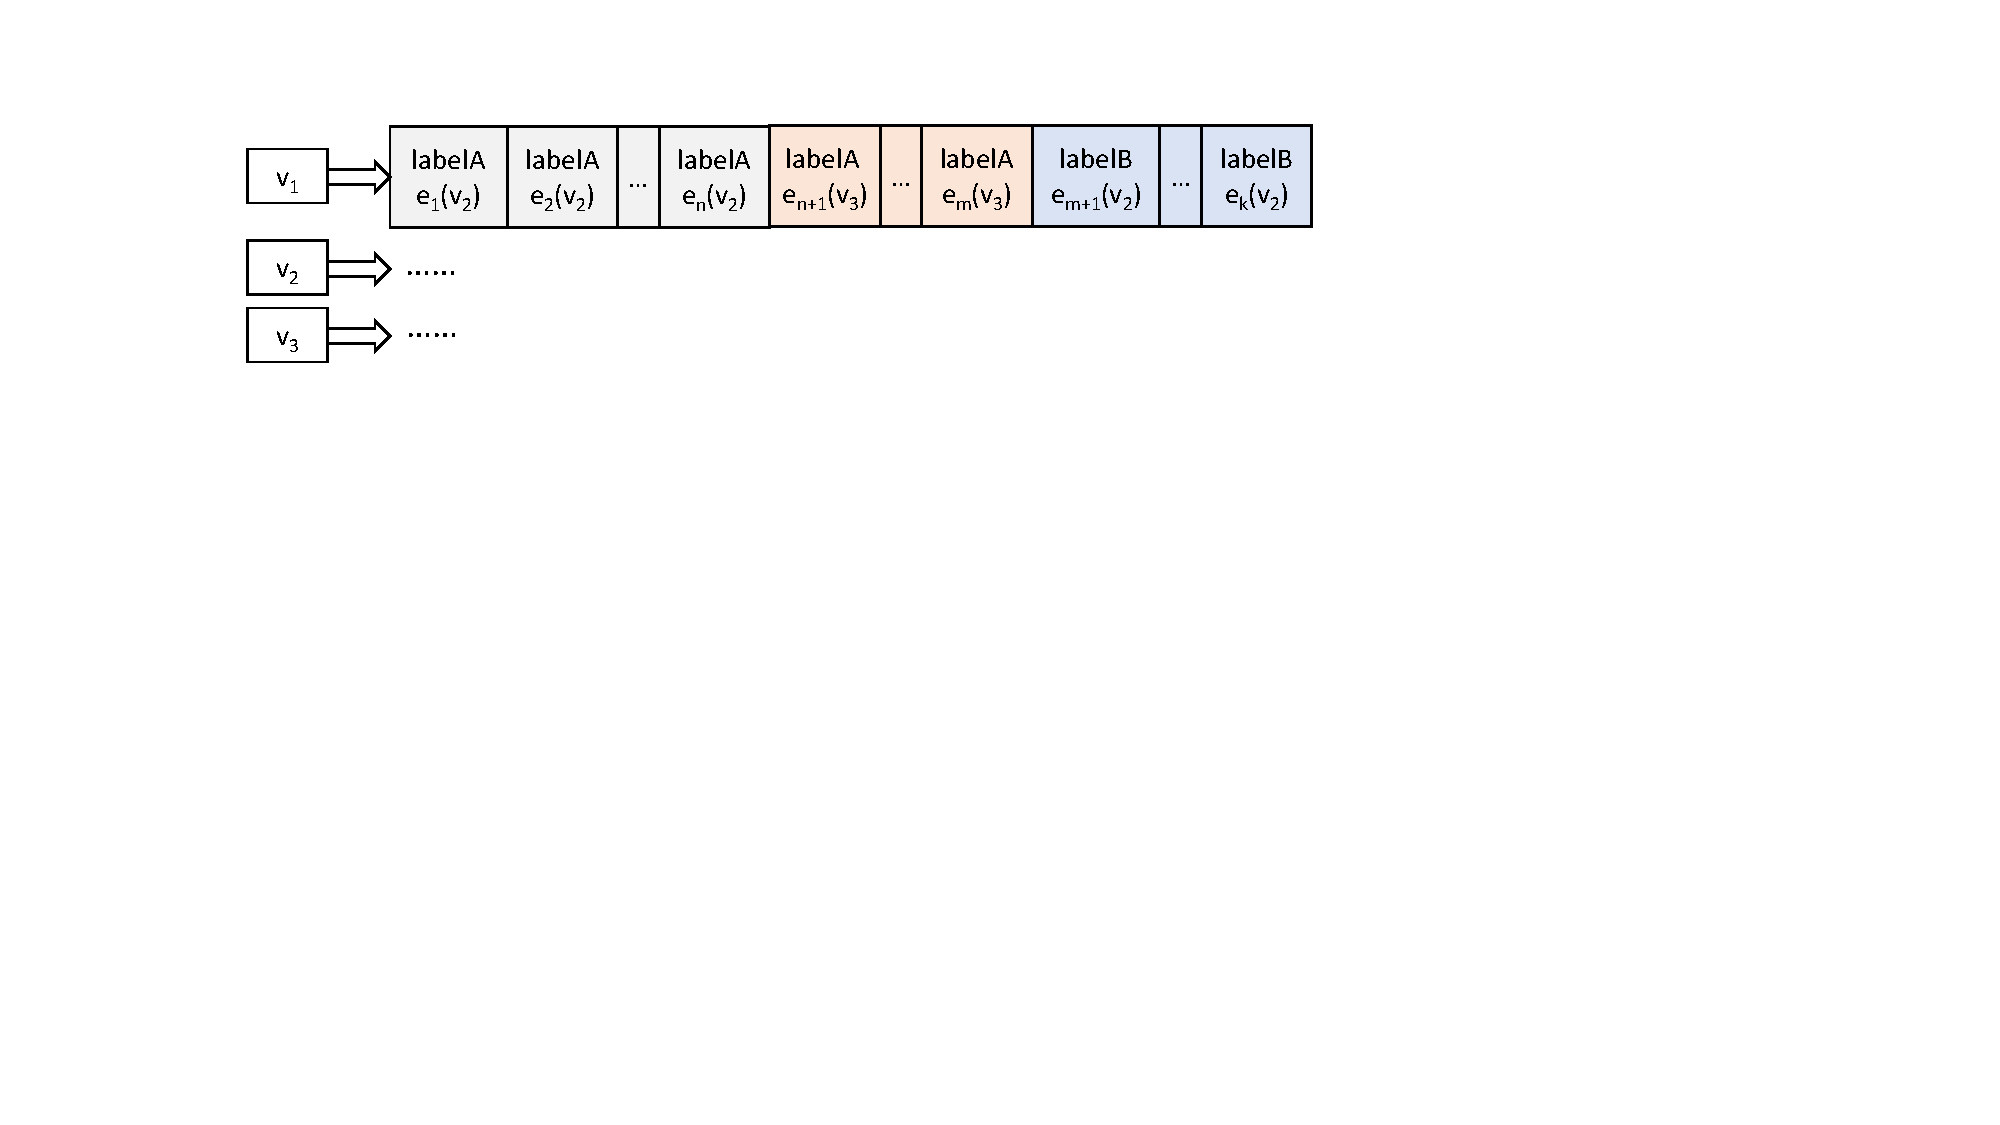
\includegraphics[width=150mm]{fig/original_list.pdf}
\caption{当属性图富含重边时,Titan在HBase中的数据表是一张扁平而宽的表}
\label{fig:orginal_list}
\end{figure}

图\ref{fig:orginal_list}展示了富含重边时邻接表的示例,为方便展示省略了边的方向。v1只有v2和v3\\
两个邻接点,其中与v2有两种label的边,与v3有一种label的边。虽然邻接的点数不多,但v1与邻接点都有数量巨大的重边。由于邻接表存储的是每条边的信息,当要查询v1的所有邻接点集(即v2、v3)时,不得不遍历一次v1的所有边,即遍历整行数据。类似地,如果要查询v1与v2的所有边时,由于这些边存储位置不相邻,也只能遍历整行数据再做过滤。

为了规避上述情形,我们可以换一种列名设计来优化邻域点集查询,比如让邻接表先按邻接点id排序,令
\begin{equation}
  \mbox{列修饰符} = adjVid + \mbox{边}label + \mbox{方向} + eid \label{eq:cq_redesign}
\end{equation}
上式与式\ref{eq:cq_design}的区别是把邻接点id(adjVid)移到了第一部分,对应的邻接表变为图\ref{fig:redesign_list}所示。此时优先按邻接点来排序,其次再按边label进行排序。因此邻接点为v2的边现在都排在了一起,可以通过一次scan全部读取出来,不需要再读取整行数据。这样在查询邻接点时,还可以跳过相同邻接点的所有边,不用再遍历整个邻接表。

\begin{figure}[htbp]
\centering
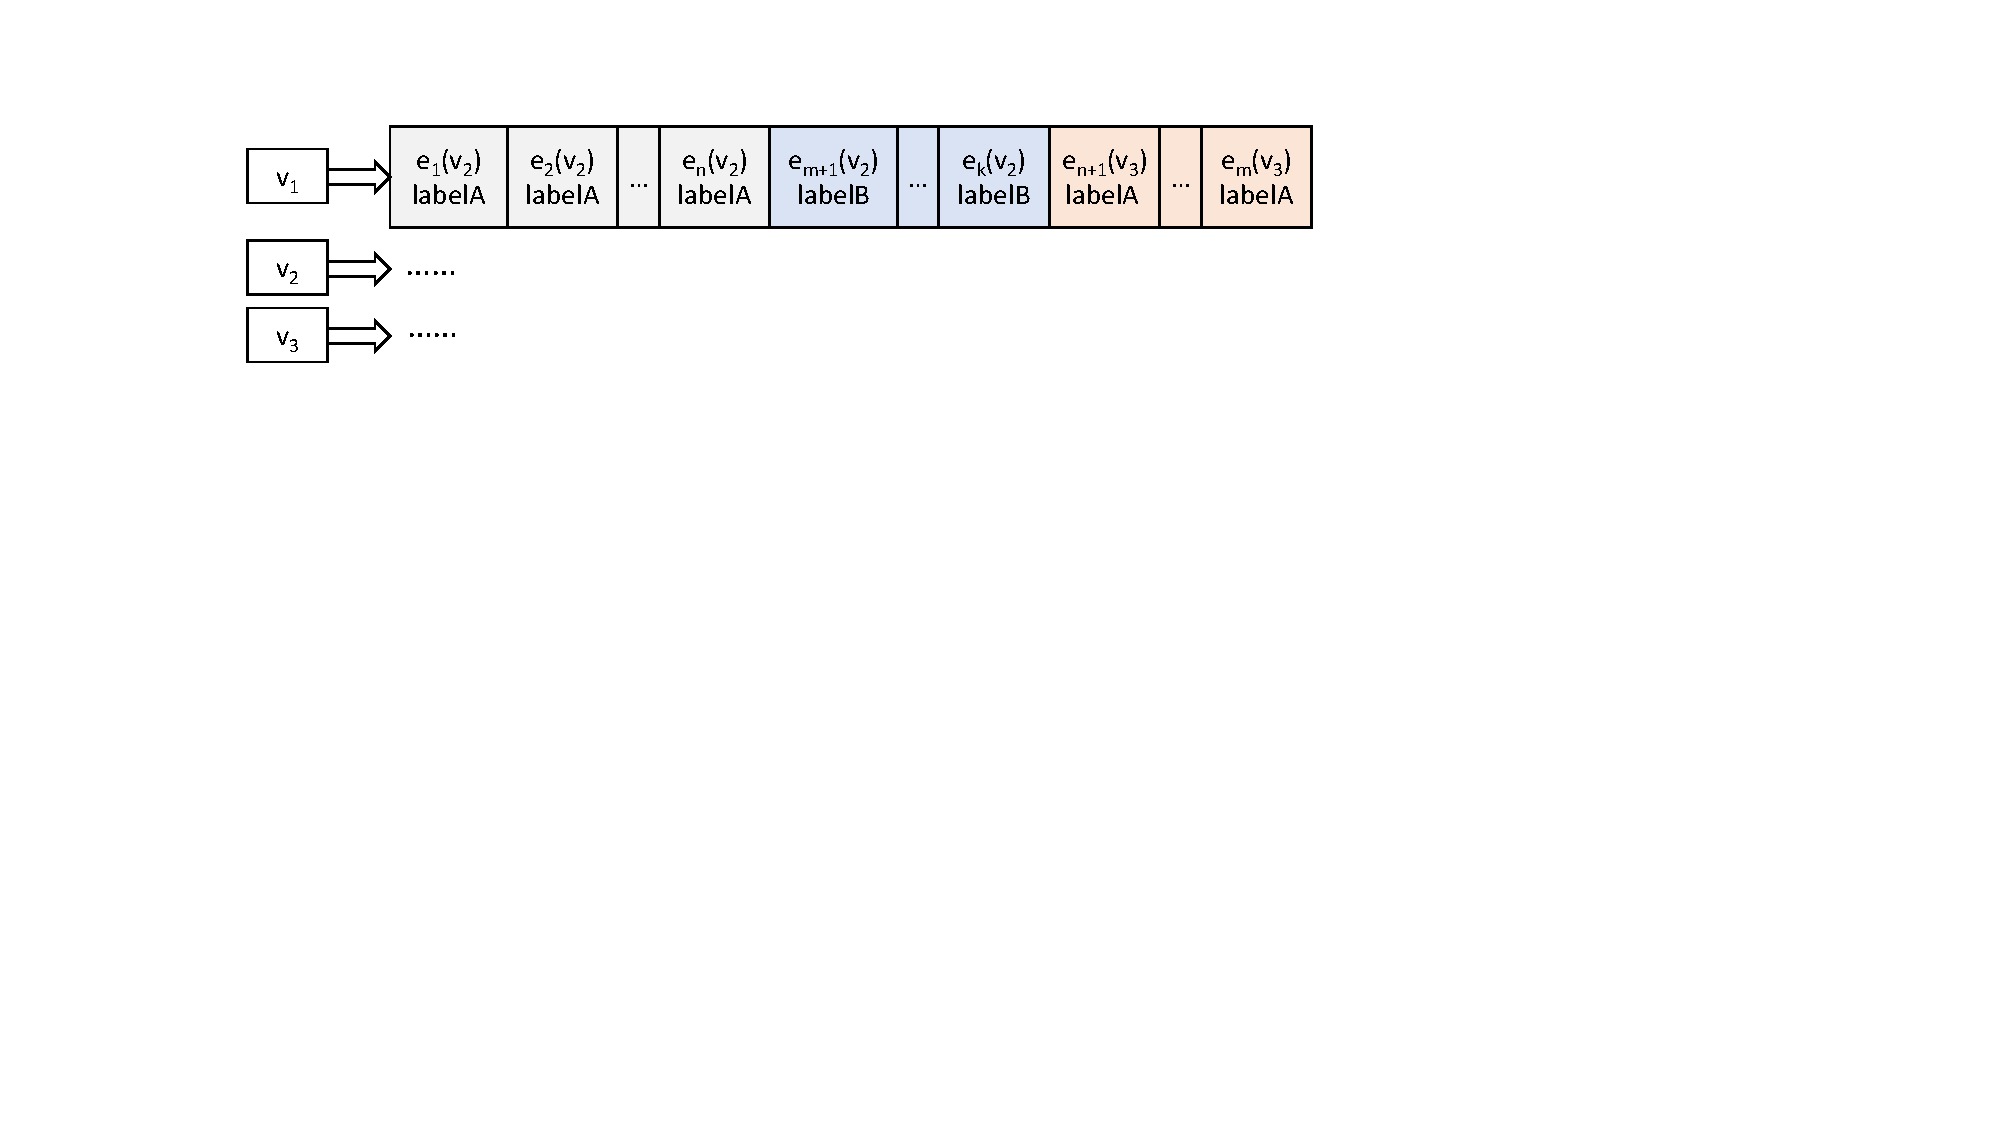
\includegraphics[width=150mm]{fig/redesign_list.pdf}
\caption{重新设计的列修饰符对应的邻接表示例}
\label{fig:redesign_list}
\end{figure}

然而,面对label相关的查询时又会面临同样的问题,比如查询该点总共有几种label的边,或者查询该点某种label的边,仍会面临原来的情形,需要遍历该点的整个邻接表。因此,改变邻接表的列名设计并不能解决问题,本质原因是邻接表存储了所有的边集。不管如何设计列修饰符,对于限定条件不包含列修饰符首位的查询,都需要遍历整行数据再进行过滤。


另一方面,当重边数量巨大时,Titan缓存的低效也影响了查询速度。Titan为加快数据访问设计了缓存,存储最近访问的点及其邻接表内容。其缓存基本上是基于HBase的 Server端Cache来实现的,即最近访问的内容会缓存在RegionServer的 BlockCache中。如果图中各点的重边都很多,则缓存空间被大量的重边占满。然而这些数据经常是与查询结果无关的被过滤数据,在做邻域相关查询时就会极大增加缓存的失效率。

\vspace{2mm}

综上总结如下,Titan在处理大量重边时查询性能急剧下降,主要原因有两方面:
\begin{enumerate}
    \item 不管列修饰符如何设计,总可以找到限定条件不包含列修饰符首位的查询,使得查询需要遍历整行邻接表
    \item 缓存中存放了大量与查询结果无关的重边数据,增加了缓存的失效率
\end{enumerate}

\vspace{3mm}

面对富含重边的属性图,把所有边集都存储在邻接表中是Titan查询性能受损的原因所在。本文基于以上分析,提出了一种基于Titan和列式存储数据库HBase的复合架构设计——HybriG。HybriG架构有如下几方面的特点:
\begin{itemize}
  \item 基于Titan和HBase建立存储层,用Titan来存储图的结构信息和点集的属性信息,HBase存储边集的所有属性信息。
  \item 在HybriG中邻接表保持了项数和数据量上的精简,从而能克服上述图数据库的缺点。
  \item 相比于传统图数据库Titan,HybriG在邻域点集相关查询以及边集数据批量导入上具有优异的性能。
\end{itemize}


% vim:ts=4:sw=4

	% Copyright (c) 2014,2016 Casper Ti. Vector
% Public domain.

\chapter{HybriG系统设计} \label{chap:design}
\section{HybriG的系统架构概述}
为了更好地应对含有大量重边的属性图应用场景,规避传统图数据库的局限性,本文提出了一种复合存储架构HybriG。
HybriG将图的连接信息和点集的属性数据存储在Titan中,边集的所有属性数据则直接存储在HBase中。由于HybriG架构基于Titan和 HBase实现存储,而Titan的数据本身也存储在HBase中,为了方便表述以及避免混淆,下文中的HBase指的都是不包含Titan数据表的部分。Titan在HBase中的数据表直接用 Titan 代称。

\begin{figure}[htbp]
\centering
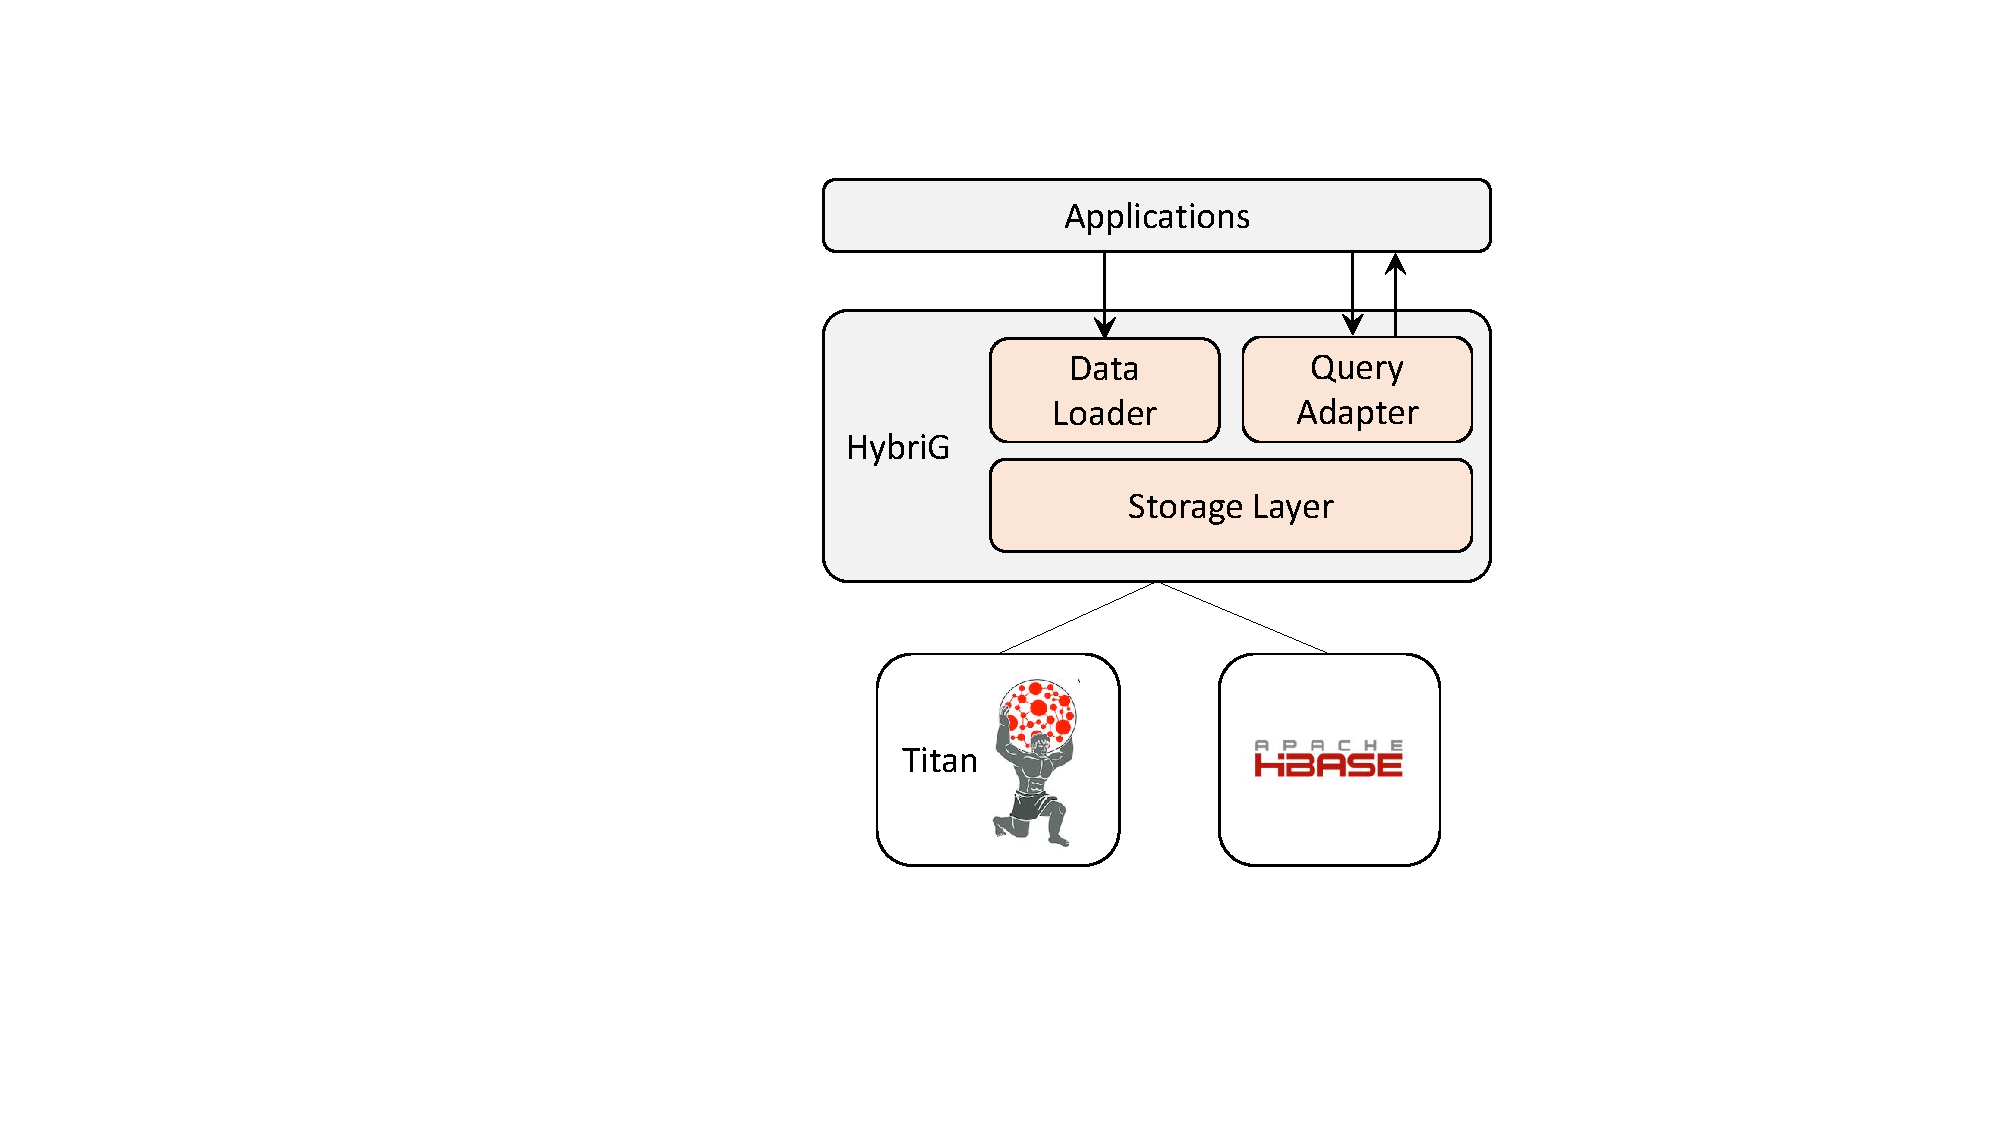
\includegraphics[height=80mm]{fig/arch.pdf}
\caption{HybriG系统架构}
\label{fig:arch}
\end{figure}

图 \ref{fig:arch}展示了HybriG的系统架构。Storage Layer是HybriG的存储层,Query Adapter和 Data Loader分别为用户程序提供图查询和数据插入接口。其中,Query Adapter将图查询转换为对Titan和HBase数据的高效查询,再将结果汇总返回给用户程序。Data Loader实现了数据的高效导入,在面对大批量的数据导入时,实现了错误恢复、断点恢复机制,同时保证了Titan和HBase的数据一致性。下面将分别介绍HybriG各模块的实现。


\section{Storage Layer}
HybriG将图数据分开存储在Titan和HBase中。具体地,如果两点之间有相同label的重边,HybriG会在Titan中这两点间建立一条该label的边,将对应重边的数据都存储在HBase中的一个表,不妨称其为边表。每条边一行,行键是Titan图中分配的边id拼接上重边的主键,单元格的值则存放具体边的内容。重边的主键是这样定义的:在两点间同label的重边中,如果有一个属性能唯一确定一条边,则选该属性作为主键。比如交易关系的时间戳,两个人在同一个时间点只能发生一次交易,因此该时间戳可以唯一确定两人间的一次交易。如果某种label的边没有属性能唯一确定一条重边,则选该数据插入的时间戳作为主键。

在HBase边表中,同label的重边数据的行键都有相同的前缀(即Titan中的边id),由于HBase中的数据是按行键排序的,它们在HBase中有相邻的位置。同label的重边经常会被同时检索,这种设计使得一次顺序扫描便可得到所有同label的重边。另外,HybriG利用Titan中边上的属性记录一些统计信息,如原图中实际有几条这样的重边,或者边上某个属性值的求和等,这些统计信息可以根据业务定制,用来加快业务相关的查询,不用再遍历相关的边。

\begin{figure}[htbp]
\centering
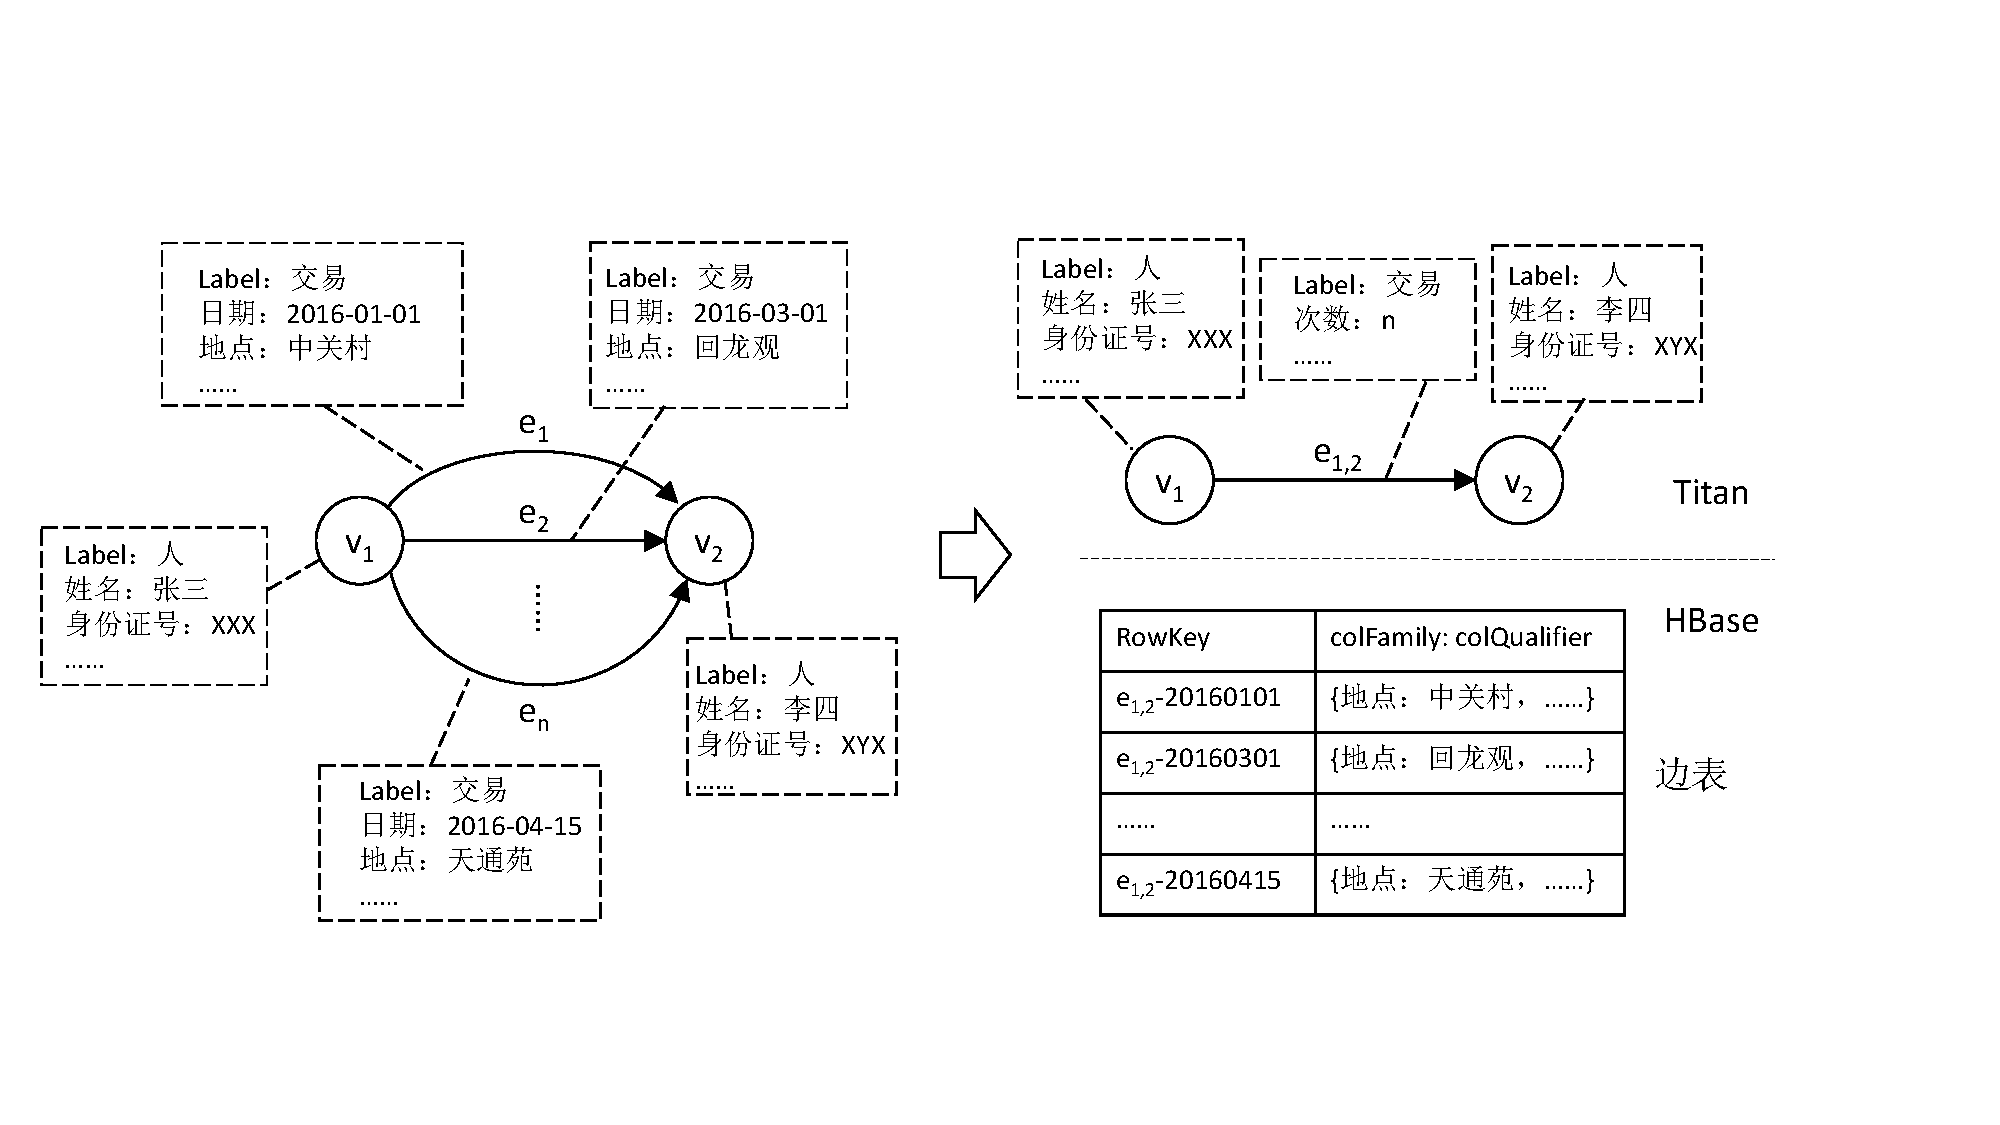
\includegraphics[width=150mm]{fig/storage_layer.pdf}
\caption[HybriG存储示例]{HybriG存储示例。左图为原始数据的属性图,右图为数据在Titan和HBase边表的存储情况。}
\label{fig:storage_layer}
\end{figure}

图 \ref{fig:storage_layer}是数据存储的一个示例,左边是实际要存储的图数据, e1、e2、…、en都是label为“交易”的重边,表示两人的所有交易记录。右边是数据在Titan和HBase中的存储情况。Titan中只存一条label为“交易”的边,该边有一个属性记录实际的边数。利用这条边的id作为前缀,拼接上重边的主键(交易的时间戳)作为HBase的行键,将每条边的数据都存入对应的单元格中。

本文在引言中提到了一种避免产生重边的建模方式,即将所有同label的重边合并为一条边来表示,边上存储这些重边的所有数据。HybriG架构与其有相似之处,但本质区别是边集元素的数据粒度仍是每条重边,不会将多条重边的数据作为一个单元来处理。在HybriG中每条边的数据独占HBase边表中的一行,因此每条边的相关操作都会更加高效。得益于HBase的高可扩展性,这种存储方式的性能也不会受制于数据规模的增长。而前述建模方式将所有重边的数据合并在一条边中存储,当重边量级巨大时,对每条边的操作势必更加低效。

\begin{figure}[htbp]
\centering
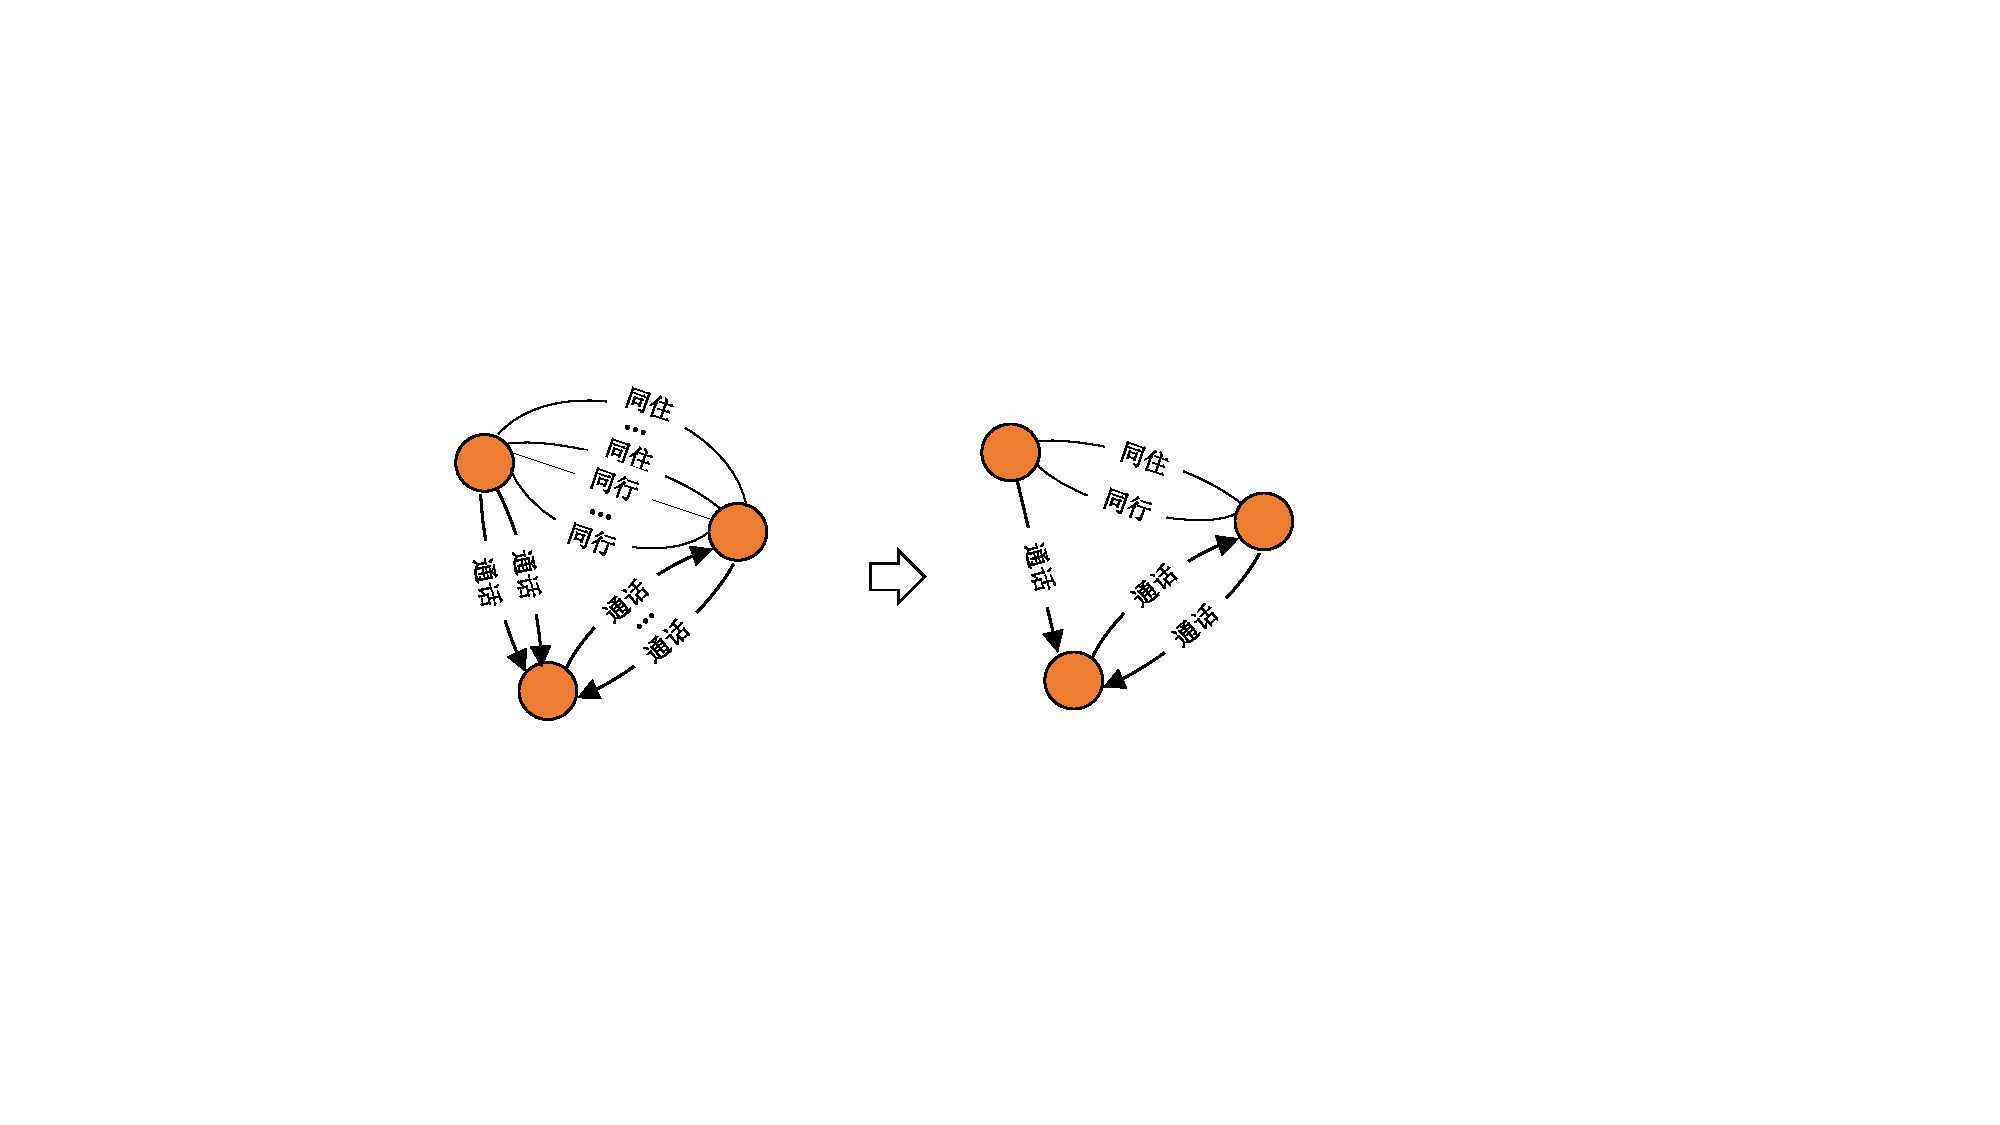
\includegraphics[width=100mm]{fig/merge_edges.pdf}
\caption[合并同label重边示意图]{合并同label重边示意。左图为实际数据图,右图为Titan中的存储示意图。无向边中的重边是指端点对应相同的两条或多条边,有向边中的重边是指起点和终点对应相同的两条或多条边。}
\label{fig:merge_edges}
\end{figure}

HybriG采用的是合并同label的重边,而不是所有的重边,这仍是基于数据粒度的考虑。图\ref{fig:merge_edges}是合并相同label重边后Titan的图示例(在HBase边表中的重边数据未显示)。在实际应用场景中,经常需要根据具体的关系种类(label)来进行邻域点集查找,对于具体边数据的查询也常按label进行。因此合并相同label的重边设计可以使很多查询在Titan中就得到满足,不需要再涉及HBase边表。


\section{Query Adapter}
Query Adapter模块将图查询转化为对应Titan和HBase的查询,再将结果汇总返回。下面分别叙述其查询设计、查询实现以及查询优势。
\subsection{查询设计}
我们在HybriG架构上实现了基本图查询接口,暴露给上层应用的仍是一张属性图。基本的图查询接口可分为如下几类:
\begin{itemize}
	\item 以点为中心的查询:获取某点邻接的点、获取某点的属性、获取某点邻接的边等;
	\item 以边为中心的查询:获取某条边的端点、获取某条边的属性等;
	\item 从图中直接查询:查询符合某种条件的元素(点/边),其中的条件可以是label、限定返回集大小(limit)等。
\end{itemize}
更详细的属性图查询接口,可以查看Blueprints中的定义。

除了基本的属性图查询接口,HybriG还提供了重边的统计信息查询。比如查询两点间某种label的重边具体的边数、或者查询某个属性上的聚集信息(如MIN、MAX、AVG、SUM等),可以根据业务需要来定制具体统计的信息。比如通话关系所表示的边中,有记录通话开始时间戳的属性。可以设置HybriG统计该类重边在该属性的最小值,从而可以查询两人最早的通话发生时间。在HybriG架构中,这些统计信息存储在Titan中的边上,因而可以快速返回结果,无需再对具体的边数据(存在HBase边表中)进行统计。

区别于传统Titan图数据库,我们没有实现事务性的接口,如newTransaction、 commit 和 rollback 等。因为业务场景可以规避对事务性的依赖,在富含重边的应用场景中,边集数据都是事件记录类型的数据,数据导入后就无需修改。而且数据导入可以分批定期执行,不会有多数据源写入导致的写-写冲突或读-写冲突。另外HybriG的数据分开存储在Titan和HBase两个数据库中,实现严格事务的代价比较大,会带来显著的性能牺牲。如Google的 Percolator\supercite{percolator} 在 BigTable 上实现了分布式事务,但写性能有75\%的牺牲。

\subsection{查询实现}
查询的实现可分为两部分,一部分只依赖于Titan中的数据,另一部分需要联合Titan 和 HBase边表的数据来返回结果。下面分别叙述。
\subsubsection{仅依赖Titan数据的查询}
在HybriG架构中,点集和各点的邻接信息都存储在Titan中,因此只与点集相关的查询都可以直接转换为对Titan的查询,如点上属性的查询、查询给定点的邻域点集、在图中查询某种label的点等。

对于重边的统计信息查询,其需要的统计结果都已在Titan的边中存储,故可以直接转换为对Titan边上的属性值查询。具体实现中需要维护一个映射关系作为元信息,以得知一个统计信息对应Titan边上的哪个属性。
\subsubsection{关联Titan和HBase数据的查询}
当查询具体的边数据时,就需要关联Titan和HBase来实现查询。在HybriG架构中,
$$HybriG\_Edge = TitanEdgeID + HBaseRowData$$
上式表示每条边对象的两部分组成,所有边集数据存储在HBase的边表中,每条边的数据占据一行,存储其所有属性,该行的行键是Titan中对应的边id拼接上该边的主键值。因此查询某条重边的数据,需要先在Titan中找到对应边的id,再在HBase边表中找到对应行的数据。

下面以两点间边集查询为例阐述HybriG的实现。两点间边集查询是指给定两个点,查询它们之间满足某种条件的边。比如已经从邻域查询得知v1与v2相邻,现在想得到它们之间某种label的所有边。查询的伪代码见算法\ref{alg:edge_query}.
\begin{algorithm}
\caption{两点间给定label的边集数据查询伪代码}
\label{alg:edge_query}
\begin{algorithmic}[1] % 每1行显示一个行号
\REQUIRE 点v1,点v2,eLabel
\ENSURE 两点间的所有符合条件的边集数据

\STATE e = v1.query().adjacent(v2).label(eLabel)
.limit(1).edges().next()
\IF{e == null}
\RETURN null
\ENDIF
\STATE res = hbaseTable.scan(e.id, next(e.id))
\RETURN wrapEdges(res)
\end{algorithmic}
\end{algorithm}

算法\ref{alg:edge_query}中,第1行查询两点间该label的边,并利用limit(1)修饰来加速,在HybriG架构中,Titan只在这两点间存储该label的一条边,因此我们可以利用边的唯一性来加速查询。第2-4行,若在Titan中查询到该label的边不存在,则不需要再在HBase中检索。第5行根据Titan中的边id,在HBase的边表中通过Scan查询得到所有边的具体数据。e.id是一个字符串,伪代码中的next(e.id)表示同等长度的下一个字符串,即将字符串e.id中最后一个字符的值加一。比如e.id为“abbb”,则next(e.id)为“abbc”。HBase的Scan函数返回连续的若干行数据,接收的两个参数是行键范围的起始和结束点,是一个左开右闭的区间。用e.id和next(e.id)作为该区间的左右端点,即可查询到所有行键以e.id作为前缀的数据。最后第6行wrapEdges函数将这些数据转换为具体的边对象,每行一条边。

\subsection{HybriG的查询优势}
\subsubsection{邻域点集相关查询的优势}

\begin{figure}[htbp]
\centering
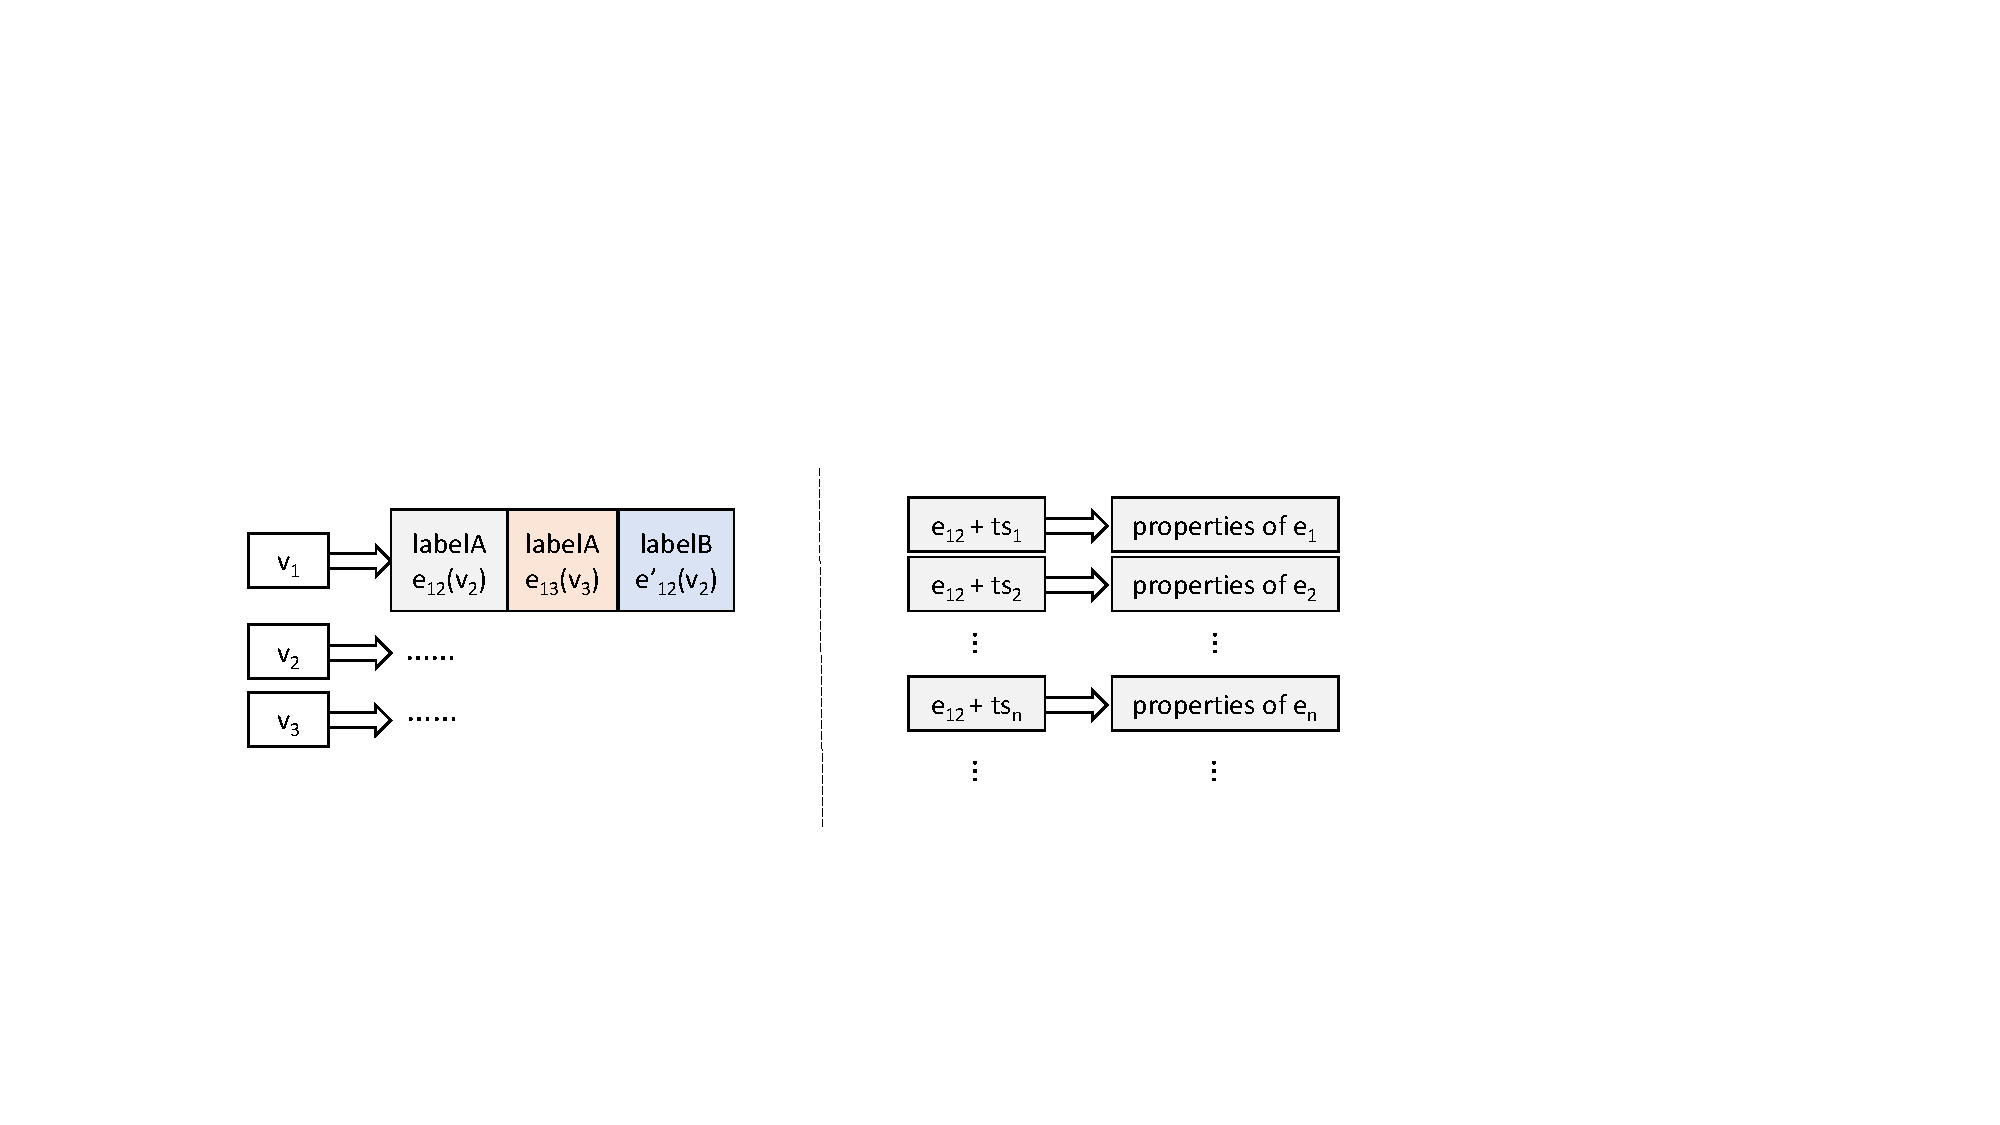
\includegraphics[width=150mm]{fig/curr_list.pdf}
\caption[HybriG在HBase中的数据表]{HybriG在HBase中的数据表分为两张,左边为Titan转化成的数据表,右边为边表。当属性图富含重边时,Titan数据表不被影响,边表将是一张高而窄的表。}
\label{fig:curr_list}
\end{figure}

为了解释HybriG在图查询上的优势,图\ref{fig:curr_list}展示了HybriG在HBase中的表结构,包括Titan自身的HBase数据表和HybriG特殊设计的边表。当属性图的重边数量爆炸性增长时,Titan的数据表并不会被影响,因为两点间同label的边至多只会存在一条,每个点的邻接表列数仍为不同label邻接的点数。另外,Titan中的边只存放统计信息,因此每个单元格(即每条边)的数据量实际很小。面对含有大量重边的属性图,各点的邻接表仍保持了列数和数据量上的精简。即使面对邻域点集查询的全表扫描,也能提供优异的性能。

另一方面,得益于邻接表的精简,Titan的缓存因此可以存放更多点集数据。对于邻域点集相关查询,如多跳邻域(k-hop)查询、路径查询、局部聚集系数计算等,具体的实现往往由多个基本的邻域点集查询组成,缓存的命中率就显得尤为重要。传统的解决方案中使用Titan存储所有的重边,使得缓存中只能存储少量点集的数据,大部分空间被边集数据占据,而具体的边集数据在查询中并不相关。在HybriG架构中,Titan的缓存能充分保留更多的点集数据,从而进一步提高邻域点集相关查询的缓存命中率。
综上,HybriG对邻域点集相关的查询具有很好的表现,后续的实验结果将展示具体的数据。

\subsubsection{边集相关查询的优势}
在许多刑侦推演场景中,往往只需要查询两点间拥是否拥有某种label的边,而不需要查看具体各个重边的数据。比如得知两人之间有共同住宿酒店的边相连后,基本可以断定两人认识,领域专家可以在图中继续推演出其他相关的人,后续有需要再展开这条关系,查看具体的各条酒店住宿记录。HybriG架构为这种场景提供了便利,上述场景相当于在HybriG架构的Titan图中进行游走(Graph traversal),当有需要时再展开某条边,在HBase边表中读回相应的边数据。

对于边集数据的读取,HybriG将所有边的数据存储在HBase边表中,而且每条边占一行,这使得对边的检索是行级别的检索,即在表中查找一行。传统的解决方案将重边数据都存储在Titan中,边集数据存储于各点的邻接表,而每个点的邻接表在HBase 数据表中占据一行,因此对边的检索是选定行后的列级别检索。HBase中行级别的检索要略优于列级别的检索,因此HybriG会略占优势。然而,HybriG对边的检索需要跨Titan 和 HBase 两个系统,会多一次交互的开销。实验表明,这两方面功过相抵,HybriG的边集数据查询性能与Titan相差不大。

HybriG架构在边集统计信息的查询或计算上会有很大优势。在HybriG架构中,Titan中某种label的边存在,代表原属性图中两点间拥有该label的边,具体的重边数据存储在HBase中的边表,而Titan中的边上的则存储了该label声明时设定的统计信息,如具体的重边数目、边上某个属性的最大最小值等。对于这些统计信息,可以直接在Titan中查询得到结果。


\section{Data Loader}
Data Loder模块负责图数据的导入,包括点的导入和边的导入。在HybriG架构中,点集数据都存储在Titan中,故点集数据导入直接在Titan上完成。边集数据虽然存储在HBase中,但Titan中的对应边上存储了重边的统计信息,因此需要同时更新Titan 和 HBase,以保证二者数据的一致。下面详述边的数据导入,以及如何保证Titan和HBase的数据一致性。

\subsection{边数据的高效导入}
在HybriG架构中,边的插入既要更新Titan,又要更新HBase中的边表。对于给定label的一条边数据,首先要查看Titan中两点间是否已有一条边表示这样的关系存在。若这样的边不存在,则将其创建。然后更新Titan边上的统计信息,再利用其边id将具体边的数据存入HBase中。算法\ref{alg:insert_one_edge}展示了上述逻辑。第1行查询Titan中该label的边,由于至多只有一条,故可用limit(1)加速。第2-4行若这样的边不存在,则在Titan中添加一条边。第5行根据要插入的边数据来更新Titan中边上的统计信息。第6行提交对Titan的所有修改。第7行将边数据写入HBase边表中,行键为e.id拼接上边的主键。
\begin{algorithm}
\caption{插入一条边的伪代码}
\label{alg:insert_one_edge}
\begin{algorithmic}[1] % 每1行显示一个行号
\REQUIRE Titan图接口graph,HBase边表接口hbaseTable,点v1,点v2,edgeLabel,边数据realEdge

\STATE e = v1.query().adjacent(v2).label(edgeLabel).limit(1).edges().next()
\IF{e == null}
\STATE {e = v1.addEdge(v2, edgeLabel)}
\ENDIF
\STATE updateStats(e, realEdge.properties)
\STATE graph.commit()
\STATE hbaseTable.put(e.id + realEdge.primaryKey, realEdge.properties)
\end{algorithmic}
\end{algorithm}

传统的解决方案将所有重边存储在Titan中,边数据的导入逻辑只需要上述代码的第3、5、6行。HybriG架构中每条边的插入多加了一次查询操作(第1行),以及HBase边表的插入操作(第7行),带来了额外的时间开销。而且最耗时的也是这两步操作,分别要从底层存储读取数据以及持久化所有修改到底层存储中。如果有批量重边需要导入,这些开销可以让所有重边来平摊,即在数据导入时,对于两点间同label的重边作为一批来处理,这样就可以共享查询操作的结果,对Titan边上统计信息更新的持久化操作(commit)也只需进行一次。批量导入重边数据的伪代码如算法\ref{alg:insert_batch_edges}所示。
\begin{algorithm}
\caption{重边数据的批量导入}
\label{alg:insert_batch_edges}
\begin{algorithmic}[1] % 每1行显示一个行号
\REQUIRE Titan图接口graph,HBase边表接口hbaseTable,点v1,点v2,edgeLabel,重边数据集allRealEdges

\STATE v1.query().adjacent(v2).label(edgeLabel).limit(1).edges().next()
\IF{e == null}
\STATE e = v1.addEdge(v2, edgeLabel)
\ENDIF
\FOR {realEdge in allRealEdges}
\STATE {updateStats(e, realEdge.properties)}
\ENDFOR
\STATE graph.commit()
\FOR {edge in allRealEdges}
\STATE {hbaseTable.put(e.id + realEdge.primaryKey, realEdge.properties)}
\ENDFOR
\end{algorithmic}
\end{algorithm}

在算法\ref{alg:insert_batch_edges}中,第1到8行是对Titan的更新,将两点间同label的重边作为一批处理,共享了对Titan的操作,从而平摊了额外的开销。另外第9到11行是对HBase边表的多次put操作,可以使用HBase的Bulk Loading 技术来进行加速。

\subsection{数据一致性}
在Titan的接口设计中,对图(graph)的初次操作将自动打开一个事务,执行 graph.commit() 时该事务提交,将事务里的修改持久化到底层存储中,Titan的事务保证了自身数据的一致性。HybriG架构由于把边数据的存储分开在Titan 和 HBase上,需要保证Titan和HBase上数据的一致性。比如Titan上关于重边的统计信息跟HBase边表的一致性,或者HBase边表里各行行键的边id部分跟Titan里的一致性。由于实现强一致性的代价过高,本架构保证的是Titan和HBase数据的最终一致性\supercite{eventually_consistent},即系统保证在经过错误恢复后,数据最终会达到一致的状态。最终一致性足以满足应用场景的需求。

由于只有边集数据是跨Titan和HBase存储的,下面讨论的都是边数据的导入。图\ref{fig:insert_steps}演示了边数据导入的三个步骤,第①步对应前述算法3中的第1~7行,更新Titan数据;第②步对应第8行,提交修改;第③步对应第9~11行,利用边id将边数据插入HBase边表中。对数据的持久化修改是第②③步,数据会出现不一致的原因是②③并不是原子的。如果②成功但是③失败了,即成功持久化了对Titan数据的修改,但对HBase边表的修改却失败了,则两方的数据出现不一致。失败的原因是多种多样的,比如程序内存溢出(Out of Memory)、网络中断、硬件故障等。

\begin{figure}[htbp]
\centering
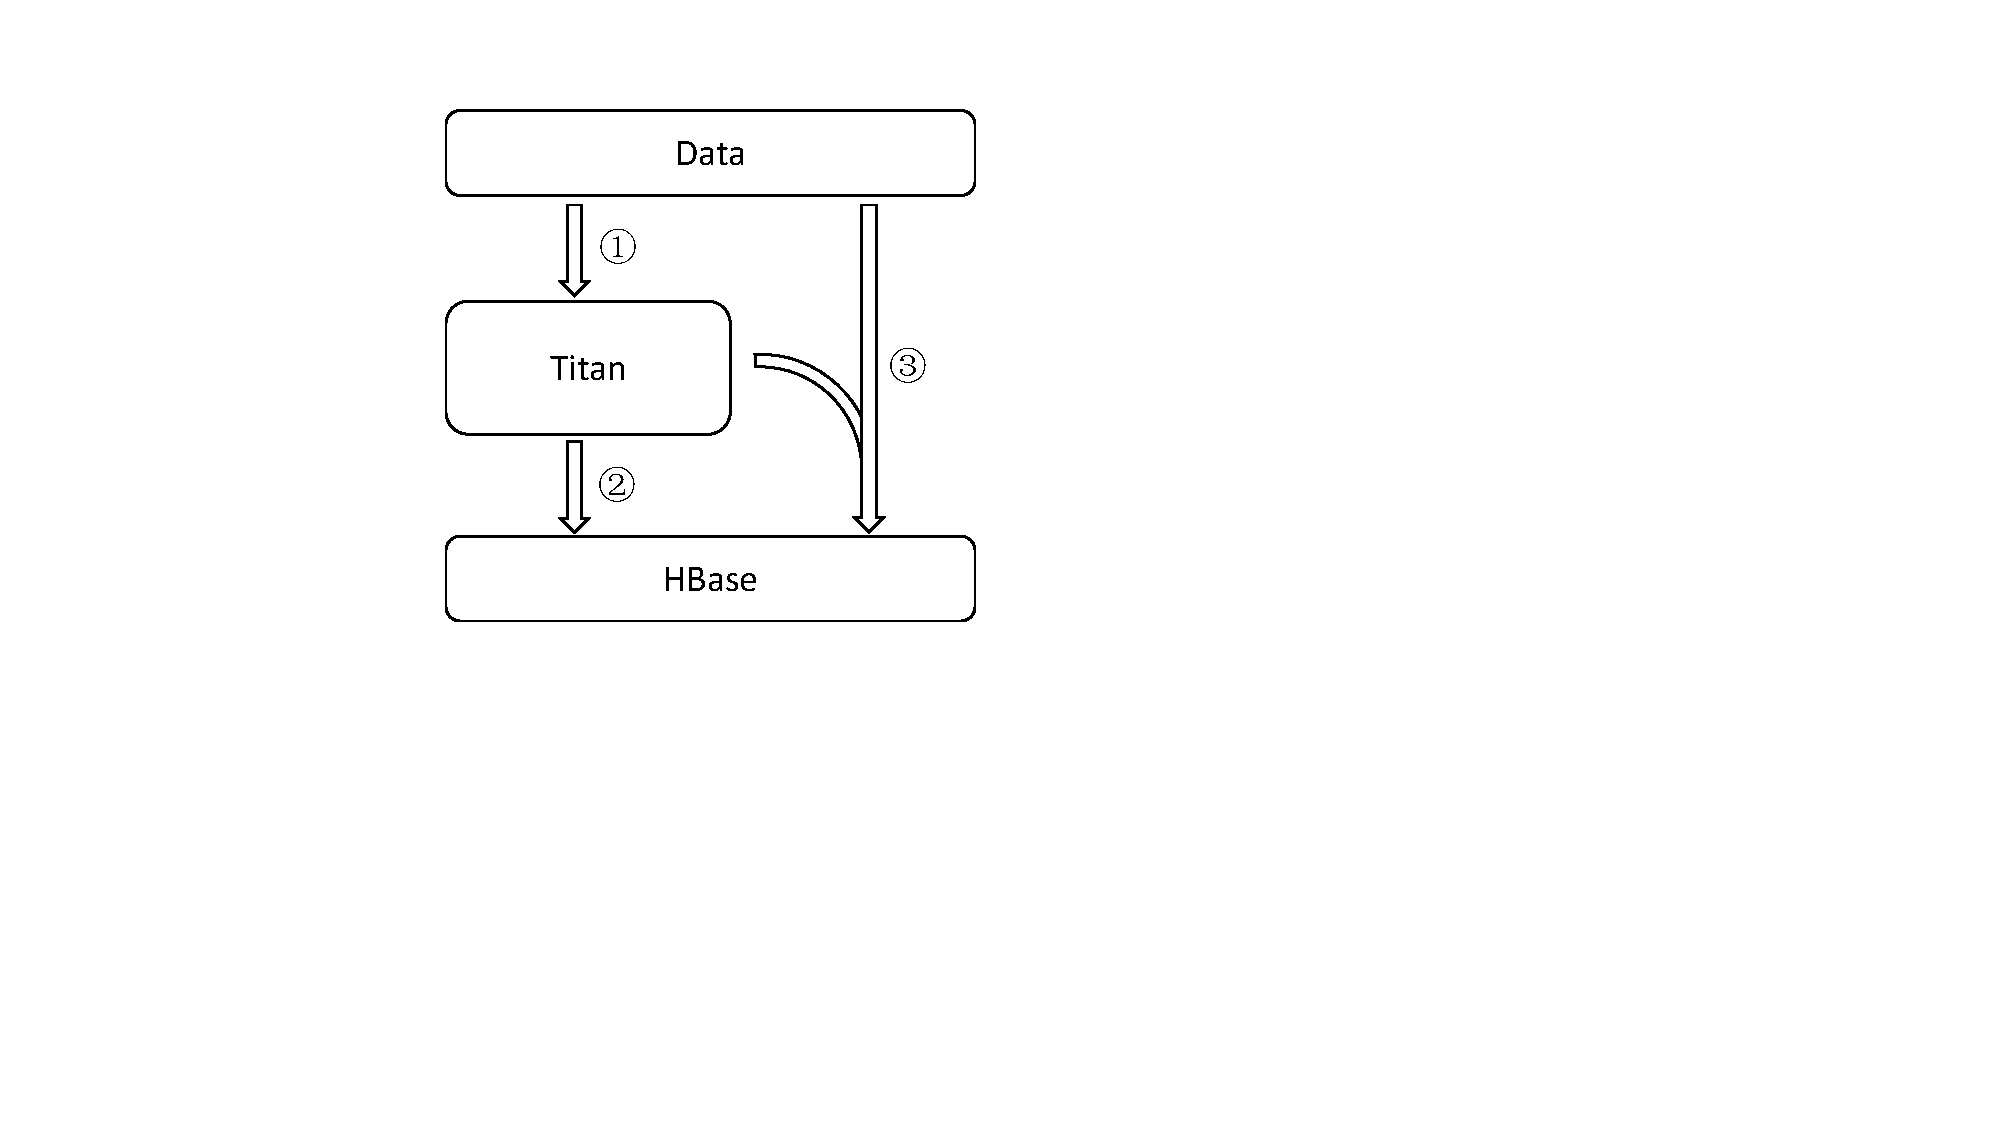
\includegraphics[width=60mm]{fig/insert_steps.pdf}
\caption[插入边数据的三个阶段]{边的数据导入分三步:①更新Titan数据;②提交Titan更改即graph.commit();③将数据插入HBase边表中}
\label{fig:insert_steps}
\end{figure}

当数据导入程序在故障之后重启时,这种不一致性需要被修复。该批次的边数据将会被重新导入,为了得知②是否已经成功,我们需要知道Titan中的数据是否已经被修改了。这可以利用Titan的
事务原子性来实现:在②提交之前,往Titan中写入一个成功标志(可以用一个点或属性来表示),然后再提交。根据原子性,该标志被成功写入当且仅当Titan的更新都被持久化。这样当数据导入程序重启时,我们先查看该标志是否存在,便可得知②是否已经成功了。若其已成功,则跳过这一步,直接进行第③步。该过程的伪代码如算法\ref{alg:consistence}所示。

\begin{algorithm}
\caption{保证一致性的边集数据批量导入}
\label{alg:consistence}
\begin{algorithmic}[1] % 每1行显示一个行号
\REQUIRE graph,batchID,HBase边表hbaseTable,点v1,点v2,edgeLabel,allRealEdges,所有边的属性
\STATE e = v1.query().adjacent(v2).label(edgeLabel).limit(1).edges().next()
\IF {hasNotCompleted(graph, batchID)}
	\IF {e == null}
		\STATE {e = v1.addEdge(v2, edgeLabel)}
	\ENDIF
	\FOR {realEdge in allRealEdges}
		\STATE {按需更新边上的统计信息}
	\ENDFOR
	\STATE markCompleted(graph, batchID)
	\STATE graph.commit()
\ENDIF
\FOR {edge in allRealEdges}
	\STATE {hbaseTable.put(e.id + edge.pk, properties)}
\ENDFOR
\end{algorithmic}
\end{algorithm}

算法\ref{alg:consistence}中,第2行的函数hasNotCompleted判断给定的Titan图中是否存在给定批次的成功标志。若不存在则执行第3到10行更新Titan,其中第9行的markCompleted函数在Titan图中插入该批次的成功标志。

值得一提的是,我们在HBase中并没有放置成功标志。如果数据导入程序在第③步成功插入HBase数据后出现故障,则重启后还会将边集数据再次插入HBase中。但这是没有问题的,因为HBase边表中的数据不存在统计信息,因此不存在更新操作,所有操作都是新数据的插入操作。我们设置HBase的最大版本数为1,则多次插入同一内容到一个单元格,实际只保存一份,不会增加存储开销。


% vim:ts=4:sw=4

	% Copyright (c) 2014,2016 Casper Ti. Vector
% Public domain.

\chapter{实验和分析}
在现有的公开数据集(比如LDBC 、SNAP 、LAW )中,并没有富含重边的场景,这些图也不是属性图。富含重边的属性图普通存在于电信、金融、刑侦等行业中,数据是不公开的。由于实际的数据只能在相关部门内部查询,明略数据根据客户数据中统计出的特征构造测试用图,以支持SCOPA的开发与测试,验证HybriG架构的优秀性能。

本组实验选用的图中有20万个顶点,48197700条边,平均度数为482,每个点平均与3.6个点相邻,两点间同label的重边的平均重数为134。实验对比的是直接将图存储在Titan中的传统方案以及将图存储在HybriG中的方案。

实验环境为5台服务器组成的集群,每台机器安装Ubuntu14.04操作系统,物理配置均为一个Intel Xeon E3-1220 (3.10GHz)处理器、16GB内存、一个1Gbps网卡及一个4TB SATA接口硬盘。HBase部署在这5台机器上,每台机器的RegionServer设置最大堆内存为4GB。其中HBase版本为1.0.1.1,Titan版本为0.5.4。

\section{邻域点集相关查询}
邻域点集查询是指查询给定点的邻接点集。许多图查询基于邻域点集查询实现,如k-hop点集查询、局部聚集系数查询、广度优先搜索等。下面叙述两个基于邻域点集查询的图查询实验。
\subsection{k-hop点集查询}
k-hop点集查询即查询给定点在k跳能到达的点集。实验在测试图中随机抽取100个点作为起点,查询它们的多跳邻域点集,测试它们的平均查询时间。同时又对小邻域(邻域点数小于5)的点集和大邻域(邻域点数大于20)的点集进行了同样的实验。表\ref{khop_random}、表\ref{khop_min}、表\ref{khop_max} 是Titan与HybriG的性能表现。
\begin{table}[!hbp]
\centering
\begin{tabular}{|c|c|c|c|c|}
\hline
\diagbox{架构}{hops} & 1 & 2 & 3 & 4\\
\hline
Titan&13.65&72.97&446.34&2755.86\\
\hline
HybriG&4.25&18.73&34.69&99.78\\
\hline
\end{tabular}
\caption{随机选100个点的k-hop查询平均耗时(毫秒)}
\label{khop_random}
\end{table}

\begin{table}[!hbp]
\centering
\begin{tabular}{|c|c|c|c|c|}
\hline
\diagbox{架构}{hops} & 1 & 2 & 3 & 4\\
\hline
Titan&8.67&31.08&179.47&1140.0\\
\hline
HybriG&2.08&7.79&19.88&52.45\\
\hline
\end{tabular}
\caption{随机选100个小邻域点的k-hop查询平均耗时(毫秒)}
\label{khop_min}
\end{table}

\begin{table}[!hbp]
\centering
\begin{tabular}{|c|c|c|c|c|}
\hline
\diagbox{架构}{hops} & 1 & 2 & 3 & 4\\
\hline
Titan&17.79&110.34&721.25&4781.79\\
\hline
HybriG&3.52&14.49&39.98&163.15\\
\hline
\end{tabular}
\caption{随机选100个大邻域点的k-hop查询平均耗时(毫秒)}
\label{khop_max}
\end{table}
可以看到,随着跳数的增加,两系统的查询时间都呈指数增长。HybriG不管在1跳的初始值还是在增长的倍数上都远优于Titan。正如2.3节分析的,对某个点的邻域点集查询需要遍历该点的邻接表。当图中的重边数目巨大时,Titan受累于其庞大的邻接表,对邻域点集的查询速度大大降低。而HybriG由于极大简化了存储在Titan中的边数目,使得邻接表的数据量大大缩小,从而降低了邻接表的遍历耗时。

\subsection{局部聚集系数计算}
局部聚集系数(Local Cluster Coefficient)是图中每个点的一种度量,用于表示其邻域子图的紧密程度,即邻居节点之间有多大比例有边相连。简要的计算公式如下:
$$LCC(v) = \frac{\left | \left \{(u,w):u,w \in{N_v}, e(u,w)\in{E} \right \} \right |}{\left | \left \{(u,w):u,w\in N_v\right \} \right |}$$
其中$N_v$表示点$v$的邻域点集,$E$表示图中的边集。上式表示邻域的点对集合中,有边相连的点对比例。由于$e(u,w)\in{E}$等价于$w\in{N_u}$,故上式分子部分可转化为
$$\left | \left \{ (u,w):u,w\in{N_v},w\in{N_u} \right \} \right | = \sum_{u\in{N_v}}{\left | N_u \cap N_v  \right |}$$
从上式可知,局部聚集系数的计算需要对邻域点集中的点再做一次邻域点集查询,因此其复杂度相当于2跳邻域点集查询。

\begin{figure}[htbp]
\centering
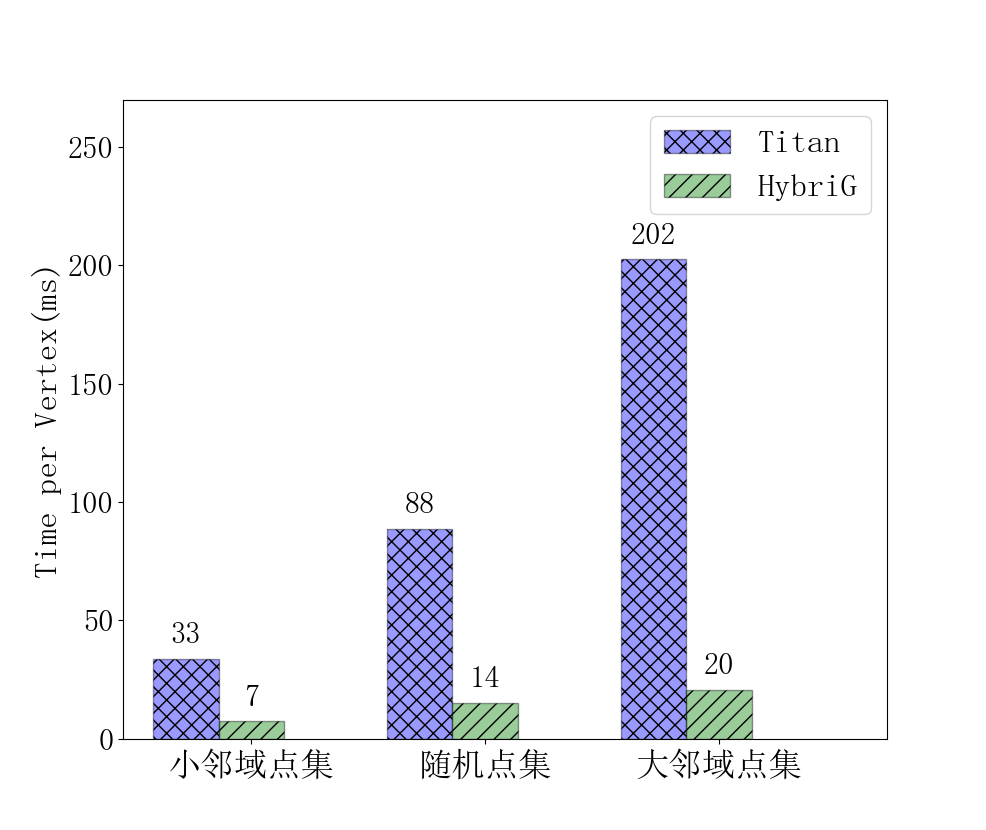
\includegraphics[width=120mm]{fig/local_cc.png}
\caption{计算100个点的局部聚集系数的平均耗时}
\label{fig:local_cc}
\end{figure}

实验对比的是HybriG与直接将图存储在Titan中的传统方案。测试点集的抽取方式同7.1节,即小邻域(邻域点数小于5)的点集、随机采样点集和大邻域(邻域点数大于20)的点集,每个点集拥有100个点。图\ref{fig:local_cc}是实验结果。
与k-hop查询一样,HybriG在局部聚集系数计算的性能上要远优与Titan,而且在大邻域点集上的优势更加明显。

\section{边集相关查询}
下面介绍边集相关查询的两个实验结果。7.2.1节是两点间边集查询,在刑侦场景中,图中的一类顶点代表人,人之间的边代表两人的关系,比如共同出行记录、共同住宿酒店记录、通话记录等。当研判专家锁定两个嫌疑人后,需要查询两人间的关系数据,即为两点间边集查询。7.2.2节是邻接边集查询,在刑侦场景中,锁定嫌疑人后要查看其某种类型的关系数据,即为邻接边集查询。这两种查询的图查询语句是不同的,前者限定了边的两个邻接点,后者只给定了边一个端点,侧重于限定label。使用Blueprints图查询接口,两点间边集查询的示例语句如下:
\begin{center}
  v1.query().adjacent(v2).edges()
\end{center}
邻接边集查询的示例语句如下:
\begin{center}
  v.getEdges(Direction.BOTH, eLabel)
\end{center}
其中v1、v2、v是顶点,eLabel是边的一种label,Direction.BOTH是常量,代表边的方向可以是入边或出边。
\subsection{两点间边集查询}
实验测试的是给定两个点和一个label,查询两点间该label的所有边。在图中随机抽取100个有边相连的点对,实验测试查询这些边的耗时。

\begin{figure}[htbp]
\centering
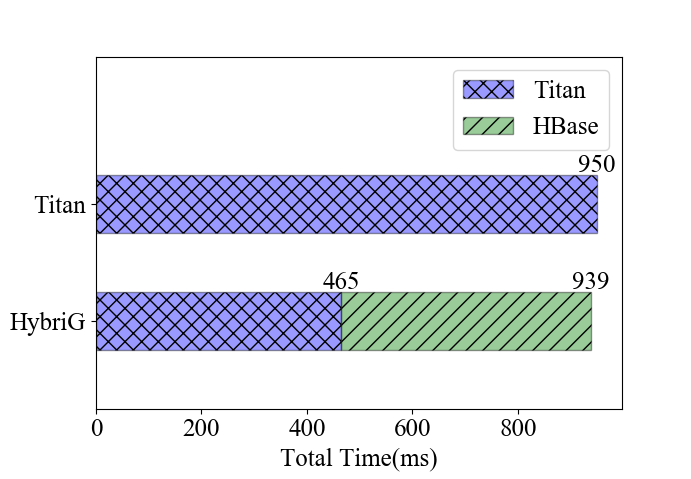
\includegraphics[width=120mm]{fig/edge_query_perf.png}
\caption{查询100个点对间所有边的总耗时}
\label{fig:edge_query_perf}
\end{figure}

图\ref{fig:edge_query_perf}统计了两种系统的时间对比,两种方案的查询耗时非常接近。HybriG的存储层基于Titan和HBase实现,对边集的查询先要在Titan里查询边id,再在HBase的边表中查询具体的边,因此时间开销分两部分(详见5.1节)。图中展示了HybriG查询时间的两部分组成。两种方案的耗时相近主要有两方面的原因。

一方面,HybriG检索边集数据需要在Titan和HBase这两个数据库中进行查询,且这两个查询不能并行。传统方案只需要在Titan中查询,HybriG多加了一轮查询的时间开销。然而,这部分的时间开销并不是很大。Titan的数据表本身也存储在HBase中,HybriG的查询实际上只是HBase中的跨表查询。跨表查询能共用HBase的一些缓存信息,如HMaster、RegionServer的位置信息、HBase中Root表和Meta表的信息等。不过尽管只是跨表查询,在这方面HybriG还是引入了时间开销。
但另一方面,HybriG对边集的查询是转化为HBase边表中的行级别检索(详见5.1节)。而将图存储在Titan中的方案,对边集的查询实际是转化为HBase数据表中选定行后的列级别检索。当图中含有大量重边时,前者是在一张高窄(tall-narrow)表中查找连续的几行,后者是在一张扁宽(flat-wide)表中选定一行后查找连续的几列,前者的性能会略优一些。因此在这方面HybriG略优。


\subsection{邻接边集查询}
实验测试的是给定一个点,查询其某种label的所有边。点集的抽取方式同7.1节,即小邻域(邻域点数小于5)的点集、随机采样点集和大邻域(邻域点数大于20)的点集,每种点集抽取1000个点。

\begin{figure}[htbp]
\centering
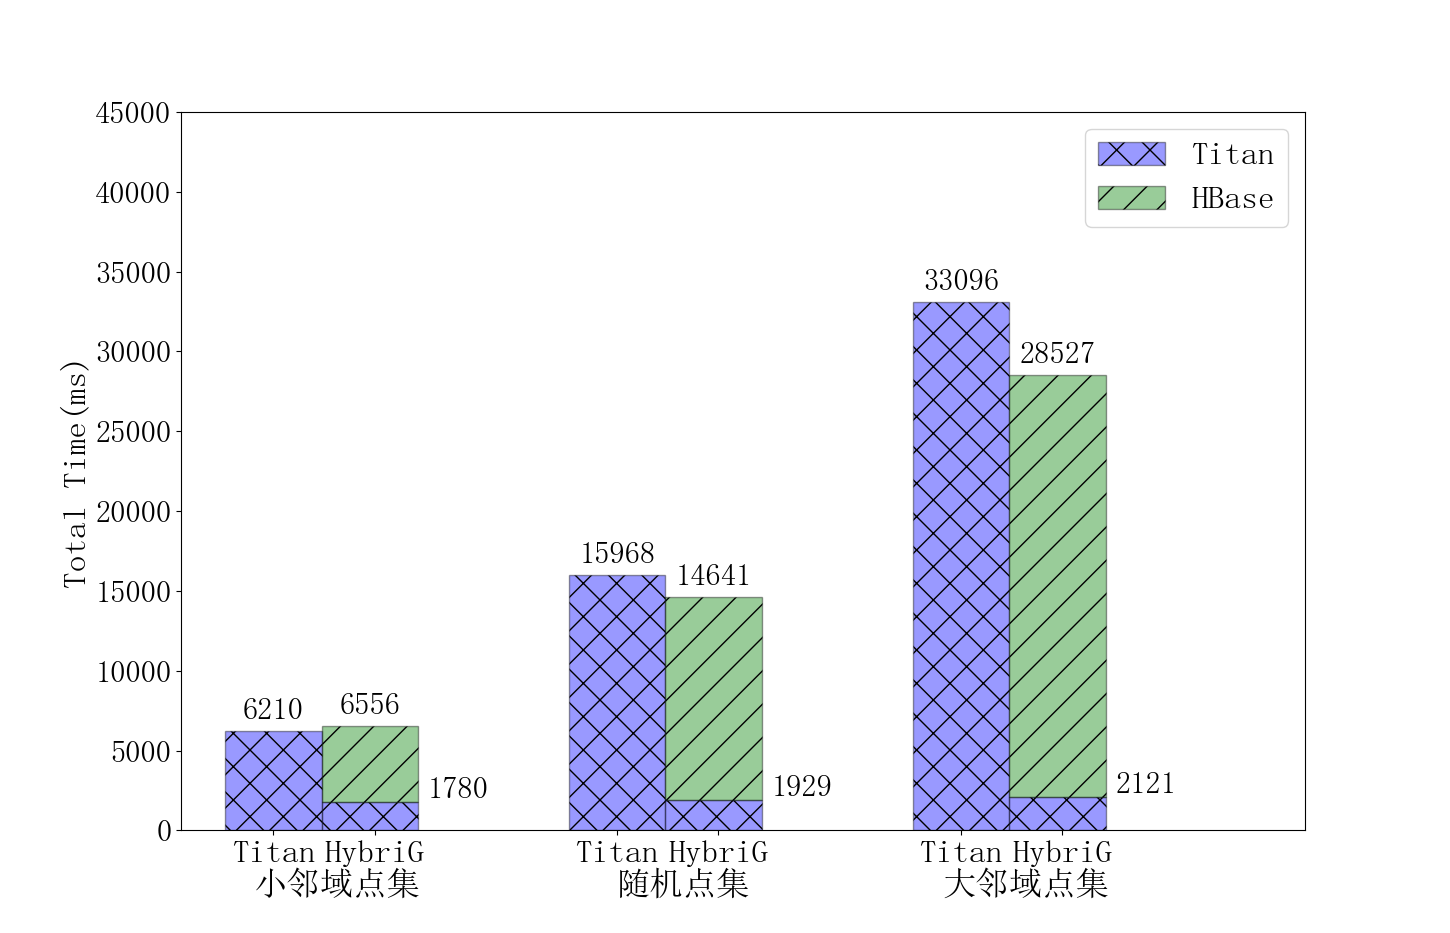
\includegraphics[width=140mm]{fig/get_edges.png}
\caption{查询1000个点给定label的所有边总耗时}
\label{fig:get_edges}
\end{figure}

图\ref{fig:get_edges}展示的是两种系统的查询时间,以及查询耗时中具体的时间组成,其中HybriG的查询时间分为Titan中的查询耗时和HBase中的查询耗时两部分。当边集规模增大时,HybriG在Titan中的查询耗时并没有显著增加,而在HBase边表中的查询耗时增长的幅度也没有传统方案中的Titan大。

\section{边数据的导入速度}
关于边的数据导入速度,我们对不同规模的图进行了测试。对比直接将图存储在Titan以及将图存储在HybriG的两种方案。我们基于MapReduce\supercite{mapreduce}开发了分布式的导入程序。表\ref{edge_load_perf}是边数据导入时间的统计:
\begin{table}[!hbp]
\begin{tabular}{|c|c|c|c|c|c|}
\hline
测试图号 & 点数 & 边数 & 重边的重数 & Titan导入时间 & HyBriG导入时间\\
\hline
1 & 50000 & 23786800 & 100 & 30min & 14min\\
\hline
2 & 200000 & 48197700 & 100 & 45min & 16min\\
\hline
3 & 200000 & 481977000 & 1000 & 9h 26min & 1h 24min\\
\hline
\end{tabular}
\caption{边集数据的批量导入耗时}
\label{edge_load_perf}
\end{table}
可以看到,在所有测试用图中,HybriG对边集数据的导入拥有更高的速度。这主要有两方面的原因:一是HybriG对HBase边表的数据导入使用了HBase的Bulk Loading技术。二是Titan对新增的点和边都会分配一个全局唯一的id(这也是Titan没有实现HBase Bulk Loading的原因),HybriG大大减小了自身Titan中的边数目,从而节省了id分配的时间开销。




% vim:ts=4:sw=4

	% 结论。
	% Copyright (c) 2014,2016 Casper Ti. Vector
% Public domain.

\specialchap{结论}
本文提出了一种基于Titan和HBase的复合存储架构——HyBriG,可以高效处理含有大量重边的属性图。相比于传统图数据库Titan的实现,HyBriG在处理大量重边时拥有更优异的查询性能,在数据导入方面也有不错的表现。

在获得高性能的同时,所带来的牺牲就是简化了对事务性的支持。然而,含有大量重边的许多应用场景并不需要很强的事务性支持,HybriG架构提供了最终一致性,足以满足这些场景的应用需求。

在实践中,明略数据的关联数据分析平台——SCOPA基于HybriG架构开发了核心存储部件。证明了HybriG架构在处理大量重边时的优异性能。


% vim:ts=4:sw=4


	% 正文中的附录部分。
	\appendix
	% 排版参考文献列表。bibintoc 选项使“参考文献”出现在目录中;
	% 如果同时要使参考文献列表参与章节编号,可将“bibintoc”改为“bibnumbered”。
	\printbibliography[heading = bibintoc]
	% 各附录。

	% 以下为正文之后的部分,默认不进行章节编号。
	\backmatter
	% Copyright (c) 2014,2016 Casper Ti. Vector
% Public domain.

\chapter{在学期间的研究成果}

\section*{发表论文}
\begin{enumerate}
    \item \textbf{黄权隆},黄艳香,邵蓥侠,孟嘉,任鑫琦,崔斌,冯是聪. "HybriG: 一种高效处理大量重边的属性图存储架构". NDBC, 2016
    \item \textbf{黄权隆},黄艳香,邵蓥侠,孟嘉,任鑫琦,崔斌,冯是聪. "HybriG: 一种高效处理大量重边的属性图存储架构". 计算机学报, 2017(已接收)
    \item Bin Cui, Jie Jiang, \textbf{Quanlong Huang}, Ying Xu, Yanjun Gui and Wenyu Zhang
"POS: A High-Level System to Simplify Real-Time Stream Application Development on Storm"
Data Science and Engineering (Springer),  1(1): 41-50, 2016
\end{enumerate}

\section*{参与的科研项目}

\begin{enumerate}
  \item 国家自然科学基金项目,61572039,支持多执行引擎的分布式图处理系统关键技术研究, 2016-2019
  \item 国家“九七三”重点基础研究发展规划项目基金,2014CB340405,网络大数据计算的基础理论及其应用研究, 2014.1-2018.12
\end{enumerate}

% vim:ts=4:sw=4

	% 致谢。
	% Copyright (c) 2014,2016 Casper Ti. Vector
% Public domain.

\chapter{致谢}

匆匆七年,就要挥手告别大学时光了。看着理一楼下的银杏又长满了绿叶,下一个赏叶的金秋自己就不在校园里了。突然有点后悔,没有过好恣意赏叶的时光。北大太美,有太多美景没来得及细品,也有太多事情没来得及完成。然而,岁月的齿轮不会回转,我们能做的终究是珍惜当下,走好未来的路。

感谢燕园赠与了我七年的美好时光。这里是一片奋斗的故土,永远忘不了通宵后松林六点钟的早餐,还有刷夜时凌晨三点的手抓饼摊。这里也是成长的地方,图书馆的走廊,邱德拔的球场,计算机系的机房,还有太多的地点,带给了我无数快乐的时光。每每走过,还能想起当初的那个自己,有过幼稚,有过自大,也有过彻悟。七情六欲,好像都能在校园里找到回忆。

最想感谢的人,是我的导师崔斌教授。或许由于缘份,大一时我的指导老师就是崔老师。崔老师治学严谨,在学术上有很强的洞察力,总能捕捉到学术前沿的发展方向,能在崔老师的指导下做研究是我们的荣幸。感谢老师的悉心指导,这些年我松懈过也努力过,感谢老师的宽容和期待。回想本科的四年,我只是在计算机领域里打了点基础;研究生的三年,才让我真正找到了专长,也愿意在这个方向继续努力下去,这些都离不开老师的指引。崔老师在学术上的孜孜不倦,将一直是我们学习的榜样。
% 还记得老师提到的全年360*10小时工作。我时常想到,追求事业就该如此。

感谢实验室的兄弟姐妹们。感谢大牛师兄姚俊杰,在我初入实验室时的悉心指导。感谢大师姐徐赢,还有土豪师姐谢怡然,小师姐黄艳香,是你们让实验室无比温馨。感谢优秀网管陈学轩师兄,以及为人随和谦逊的陈琛师兄,在读研之初,我就希望自己做人做事,能和你们相当。感谢在学术上孜孜不倦,辛苦耕耘的志师兄、邵侠、施老板和徐宁师兄,以及将要毕业的乐乐、佳伟,一直敬佩你们博士生的学术追求,从你们身上我学到了很多。感谢乐观又积极开朗的智鹏、沉着又不乏幽默的羚宇,你们为实验室带来了许多欢声笑语。还有一同度过01时光的琪姐、dk、光哥,以及本科时1631的胡志挺、陈宇望、杜焱,我会永远铭记那些美好的时光。感谢实验室的闫学灿、李旭鹏、陈一茹、苑斌、谢旭、符芳诚、李恬等各位师弟师妹,还有好多实验室的同学,不及一一细说。

感谢实习中遇到的各位同事。感谢腾讯的导师曹坤,带我养成了许多好习惯,也带领我见识到了工业界的优秀项目。感谢大师konton、Java大神大桂哥、炫酷风趣的Justy、极富学术追求的徐钊,还有精准推荐组的各位同事,暑期实习的两个月让我收获良多。感谢明略数据的冯博冯是陪、董哥董斌一直以来的看重。感谢史上最nice的leader孟嘉师兄、相声口才的任鑫琦师兄,感谢你们的信任,让我在项目中得到了真正的锻炼。感谢一起封闭开发过的同事,自带东北幽默的石海洋、爽快不羁的大哥周扬、文艺青年付骁弈、半夜打游戏但开发效率超神的李博龙,以及靠谱运维一把手闫强,我们一同经历了封闭开发,和你们合作让我收获了很多。感谢后来一起合作过的队长王啸风、为人超nice的刘泉海、老司机杨洋、有为小青年朱亚超。


最后还要感谢我的家人,感谢你们在我求学生涯里一如既往的关怀和支持。感谢我的女朋友许艺萱,我们一起成长,一起追求美好的未来。

每一段时光终会划上一个句号,感谢所有在我世界中出现过的人们,我们的人生曾有意无意地互相影响过,对此我永远心怀感恩。

% vim:ts=4:sw=4

	% 原创性声明和使用授权说明。
	% Copyright (c) 2008-2009 solvethis
% Copyright (c) 2010-2017 Casper Ti. Vector
% All rights reserved.
%
% Redistribution and use in source and binary forms, with or without
% modification, are permitted provided that the following conditions are
% met:
%
% * Redistributions of source code must retain the above copyright notice,
%   this list of conditions and the following disclaimer.
% * Redistributions in binary form must reproduce the above copyright
%   notice, this list of conditions and the following disclaimer in the
%   documentation and/or other materials provided with the distribution.
% * Neither the name of Peking University nor the names of its contributors
%   may be used to endorse or promote products derived from this software
%   without specific prior written permission.
%
% THIS SOFTWARE IS PROVIDED BY THE COPYRIGHT HOLDERS AND CONTRIBUTORS "AS
% IS" AND ANY EXPRESS OR IMPLIED WARRANTIES, INCLUDING, BUT NOT LIMITED TO,
% THE IMPLIED WARRANTIES OF MERCHANTABILITY AND FITNESS FOR A PARTICULAR
% PURPOSE ARE DISCLAIMED. IN NO EVENT SHALL THE COPYRIGHT HOLDER OR
% CONTRIBUTORS BE LIABLE FOR ANY DIRECT, INDIRECT, INCIDENTAL, SPECIAL,
% EXEMPLARY, OR CONSEQUENTIAL DAMAGES (INCLUDING, BUT NOT LIMITED TO,
% PROCUREMENT OF SUBSTITUTE GOODS OR SERVICES; LOSS OF USE, DATA, OR
% PROFITS; OR BUSINESS INTERRUPTION) HOWEVER CAUSED AND ON ANY THEORY OF
% LIABILITY, WHETHER IN CONTRACT, STRICT LIABILITY, OR TORT (INCLUDING
% NEGLIGENCE OR OTHERWISE) ARISING IN ANY WAY OUT OF THE USE OF THIS
% SOFTWARE, EVEN IF ADVISED OF THE POSSIBILITY OF SUCH DAMAGE.

{
	\ctexset{section = {
		format+ = {\centering}, beforeskip = {40bp}, afterskip = {15bp}
	}}

	% 学校书面要求本页面不要页码,但在给出的 Word 模版中又有页码且编入了目录。
	% 此处以 Word 模版为实际标准进行设定。
	\specialchap{北京大学学位论文原创性声明和使用授权说明}
	\mbox{}\vspace*{-3em}
	\section*{原创性声明}

	本人郑重声明:
	所呈交的学位论文,是本人在导师的指导下,独立进行研究工作所取得的成果。
	除文中已经注明引用的内容外,
	本论文不含任何其他个人或集体已经发表或撰写过的作品或成果。
	对本文的研究做出重要贡献的个人和集体,均已在文中以明确方式标明。
	本声明的法律结果由本人承担。
	\vskip 1em
	\rightline{%
		论文作者签名:\hspace{5em}%
		日期:\hspace{2em}年\hspace{2em}月\hspace{2em}日%
	}

	\section*{%
		学位论文使用授权说明\\[-0.33em]
		\textmd{\zihao{5}(必须装订在提交学校图书馆的印刷本)}%
	}

	本人完全了解北京大学关于收集、保存、使用学位论文的规定,即:
	\begin{itemize}
		\item 按照学校要求提交学位论文的印刷本和电子版本;
		\item 学校有权保存学位论文的印刷本和电子版,
			并提供目录检索与阅览服务,在校园网上提供服务;
		\item 学校可以采用影印、缩印、数字化或其它复制手段保存论文;
		\item 因某种特殊原因需要延迟发布学位论文电子版,
			授权学校在 $\Box$\nobreakspace{}一年 /
			$\Box$\nobreakspace{}两年 /
			$\Box$\nobreakspace{}三年以后在校园网上全文发布。
	\end{itemize}
	\centerline{(保密论文在解密后遵守此规定)}
	\vskip 1em
	\rightline{%
		论文作者签名:\hspace{5em}导师签名:\hspace{5em}%
		日期:\hspace{2em}年\hspace{2em}月\hspace{2em}日%
	}

	% 若需排版二维码,请将二维码图片重命名为“barcode”,
	% 转为合适的图片格式,并放在当前目录下,然后去掉下面 2 行的注释。
	%\vfill\noindent
	%\includegraphics[height = 5em]{barcode}
}

% vim:ts=4:sw=4

\end{document}

% vim:ts=4:sw=4
